%% This is a sample manuscript marked up using the
%% AASTeX v5.x LaTeX 2e macros.

%% The first piece of markup in an AASTeX v5.x document
%% is the \documentclass command. LaTeX will ignore
%% any data that comes before this command.

%% The command below calls the preprint style
%% which will produce a one-column, single-spaced document.
%% Examples of commands for other substyles follow. Use
%% whichever is most appropriate for your purposes.
%%

%\documentclass[11pt,preprint2]{aastex}
% manuscript produces a one-column, double-spaced document:
%\documentclass[manuscript]{aastex}
%% preprint2 produces a double-column, single-spaced document:

\documentclass{emulateapj}
%\documentclass[preprint]{aastex}

\usepackage{natbib}
\usepackage{amsmath}
\bibliographystyle{apj}
\usepackage{graphicx}

%% Sometimes a paper's abstract is too long to fit on the
%% title page in preprint2 mode. When that is the case,
%% use the longabstract style option.

%% \documentclass[preprint2,longabstract]{aastex}

%% If you want to create your own macros, you can do so
%% using \newcommand. Your macros should appear before
%% the \begin{document} command.
%%
%% If you are submitting to a journal that translates manuscripts
%% into SGML, you need to follow certain guidelines when preparing
%% your macros. See the AASTeX v5.x Author Guide
%% for information.

%% You can insert a short comment on the title page using the command below.

%\slugcomment{Not to appear in Nonlearned J., 45.}

%% If you wish, you may supply running head information, although
%% this information may be modified by the editorial offices.
%% The left head contains a list of authors,
%% usually a maximum of three (otherwise use et al.).  The right
%% head is a modified title of up to roughly 44 characters.
%% Running heads will not print in the manuscript style.

\shorttitle{The HERA Dish: Beam Measurements and Science Implications}
\shortauthors{Neben et al.}

%% This is the end of the preamble.  Indicate the beginning of the
%% paper itself with \begin{document}.

\begin{document}

\title{The Hydrogen Epoch of Reionization Array Dish I: Beam Pattern Measurements and Science Implications}

%% Use \author, \affil, and the \and command to format
%% author and affiliation information.
%% Note that \email has replaced the old \authoremail command
%% from AASTeX v4.0. You can use \email to mark an email address
%% anywhere in the paper, not just in the front matter.
%% As in the title, use \\ to force line breaks.

\author{Abraham R. Neben\altaffilmark{1},
Aaron Ewall-Wice\altaffilmark{1},
Nipanjana Patra\altaffilmark{2},
Nithyanandan Thyagarajan\altaffilmark{3},
James E. Aguirre\altaffilmark{4},
Zaki S. Ali\altaffilmark{2},
Judd Bowman\altaffilmark{3}
Carina Cheng\altaffilmark{2},
David R. DeBoer\altaffilmark{2}
Jacqueline N. Hewitt\altaffilmark{2},
Aaron Parsons\altaffilmark{2}}

\affil{\altaffilmark{1}MIT Kavli Institute, Massachusetts Institute of Technology, Cambridge, MA, 02139 USA}
\affil{\altaffilmark{2}Dept. of Astronomy, University of California, Berkeley, CA, USA}
\affil{\altaffilmark{3}Arizona State University, School of Earth and Space Exploration, Tempe, AZ 85287, USA}
\affil{\altaffilmark{4}Dept. of Physics and Astronomy, University of Pennsylvania, Philadelphia, PA}

%% Notice that each of these authors has alternate affiliations, which
%% are identified by the \altaffilmark after each name.  Specify alternate
%% affiliation information with \altaffiltext, with one command per each
%% affiliation.

%% Mark off your abstract in the ``abstract'' environment. In the manuscript
%% style, abstract will output a Received/Accepted line after the
%% title and affiliation information. No date will appear since the author
%% does not have this information. The dates will be filled in by the
%% editorial office after submission.

\begin{abstract}
THIS WILL NEED TO BE REWRITTEN
We deploy the 137\,MHz ORBCOMM beam mapping system of \citet{neben15} at the site of the HERA prototype at NRAO--Green Bank. This technique measures the beam of an antenna-under-test relative to that of a well-modeled reference antenna. We characterize environmental systematics such as reflections and multipath effects by comparing the measured beams of different reference antennas, then measure the beam pattern of the east-most HERA dish as a function of feed height over the dish surface. With the feed at the nominal focus of 4.5\,m over the dish surface, the collecting area is observed to be 68.5\,m$^2$, agreeing with simulations. We also simulate delay spectra on baselines of different lengths and orientations at different LSTs for measured and model beams, and quantify the severity of and uncertainties in the delay space horizon brightening termed the ``pitchfork effect'' by \citet{nithya15}. Future measurements will study the dish beam in the presence of adjacent dishes, quantifying levels of cross-talk and cross-coupling.
\end{abstract}

\keywords{instrumentation: interferometers --- techniques: interferometric --- cosmology: observations --- dark ages, reionization, first stars}


\section{Introduction}
%- basics of 21cm cosmology
%    - shedding light on the unobserved Dark Ages and Epoch of
%      Reionization when the first luminous sources formed and reionized
%      the IGM
%    - MWA, PAPER, LOFAR, GMRT power spectrum experiments
%    - also global signal experiments like XX,YY,ZZ,
%        - the big challenge is recovering the signal below 4-5 orders of
%      magnitude brighter foregrounds and noise
%    - naive requirement is collecting area
%    - naive foreground removal is to subtract all low $k_\parallel$ modes

A new generation of low frequency radio telescopes is coming online with the goal of
 probing redshifted 21\,cm emission from the Cosmic Dawn. These observations will 
 complement indirect probes of the Dark Ages and Epoch of Reionization such as quasar 
 sightlines, deep galaxy surveys, and the CMB optical depth which leave the reionization 
 history of the universe only loosely constrained. Sensitivity and foreground removal are 
 the main challenges in 21\,cm observations, as the expected cosmological signal is 4--5 
 orders of magnitude fainter than Galactic and extragalactic foregrounds. Radio 
 interferometers such as the MWA \citep{tingay13}, PAPER \citep{ali2015}, GMRT 
 \citep{Paciga2011}, and LOFAR \citep{lofar} are seeking a first detection of 
 cosmological 21\,cm emission in power spectrum measurements, where the smooth 
 frequency evolution of the foreground emission distinguishes itself from the spectrally 
 jagged cosmological signal whose frequency dimension is a redshift axis probing the 
 inhomogenous reionizing universe.

%%- but instrumental frequency structure has been recognized as critical
%  => wedge
%    - of course the bandpass and intrinsic smooth freq structure of
%      sources
%    - but also the freq-dependent sampling of the IFO
%    - sources at different zenith angles appear at different delays,
%      and thus different $k_\parallel$, increasing linearly with baseline length
%    - this gives rise to the “wedge” in cylindrically averaged power
%      spectra ($k_\perp$, $k_\parallel$)

It was initially thought that the foreground emission would be confined to the lowest few 
line of sight Fourier modes, however it was later realized that the spectral structure of the 
interferometer's point spread function smears foreground power into a ``wedge''-shaped 
region in  $(k_\perp,k_\parallel)$ Fourier space. The complement of this corrupted region 
is known as the ``EOR Window''. Here ($k_\perp,k_\parallel$) represent spatial modes 
perpendicular and parallel to the line of sight. This effect is straightforward to understand 
for a single baseline which measures the sky intensity weighted by the complex sky fringe 
$e^{i \vec{k}\cdot\vec{b}}$, where $\vec{k}=\vec{k}(\theta,\phi)$ is the wave vector of 
the incident radiation and $\vec{b}$ is the baseline vector in meters. A source at zenith 
has $\vec{k}\perp\vec{b}$, and so appears in the visibility without any apparent 
frequency dependence; however the visibility for a source near the horizon in line with the 
baseline is maximally frequency dependent, and proportional to $e^{2\pi i f b/c}$. 

Thus sources at different positions relative to the baseline vector manifest different 
frequency structure despite their intrinsically smooth spectra, but are geometrically limited 
by the baseline length so that maximum affected $k_\parallel$ mode is proportional to the 
baseline length, and thus to $k_\perp$. It is convenient to phrase this description in terms 
of the delay in radiation arrival at the baseline's two antennas, $\tau$, where $\tau_
\text{max}=b/c$. The interpretation is thus that sources at low delay have little frequency 
structure, while those near $\tau=\tau_\text{max}$ acquire the maximum frequency 
structure given the baseline length. 

That sources acquire frequency dependence commensurate with their position in the sky 
tells us already that the primary beam strongly affects the apparent frequency dependence 
of the foregrounds. The high delay regions of the sky lie near the horizon while low delay 
regions lie closer to zenith and also perpendicular to the baseline vector. \citet{nithya15} 
simulate the foreground contamination seen with a dipole beam, a phased array of simple 
dipoles, and a Airy dish, and find that the latter suffers minimal foreground contamination 
into of nonzero $k_\parallel$ model due to its narrow main lobe and minimal sidelobe 
levels. To be sure, all are subject to the same geometric limits on foreground frequency-
dependence, the wedge, but the emission from high delay is better suppressed using the 
Airy dish leaving much of the wedge effectively empty. 

%%- the beam affects the wedge
%    - Nithya et al quantify the effects of antenna beam on the wedge
%    - wider beams like the dipole have large response at large zenith
%      angle, and thus large delays, wedge much more filled out, and
%      much more emission close to the EOR window, at risk of leaking in
%    - narrower beams like the airy have much narrower response, most
%      received emission is from low delays (near $k_\parallel=0$)
%    - but even there, emission is seen at the edge of the wedge,
%      interpreted as an effective brightening of the horizon due to the
%      very large solid angle it subtends 
%    - this structure (lots of emission from zero delay, and peak at the
%      horizon), was termed the pitchfork
%    - highlights importance of beam characterization across the entire
%      sky

In principle, it is irrelevant how empty or full the wedge is of foreground power as it is 
perfectly contained in it, however the finite bandwidth and imperfect frequency bandpass 
of real instruments smear power beyond the geometrical edge of the wedge into the EOR 
window. Sources at higher delay appear closest to the edge of the wedge, and thus are 
most at risk of leaking into the EOR window due to these effects. In fact, 
\citet{nithya15,nithya15b} observe that while naively we might expect minimal emission 
at the very edge of the wedge because typical near-horizon beam responses are so small, 
two effects cause a relative brightening of emission at those maximal delays after the 
decline away from zero delay, creating a characteristic ``pitchfork'' shape. This horizon 
brightening is caused by the large solid angle subtended by the near-horizon regions of the 
sky, and the apparent shortening of baselines when viewed on axis at these elevations. 
This second effect makes intermediate length baselines sensitive to the very bright diffuse 
emission they would not otherwise be sensitive due to its very weak coupling to longer 
baselines. Together, these effects can over the decline in beam sensitivity near the horizon. 
All these considerations highlight the antenna beam as a critical design parameter for 
21\,cm observatories

%%- the design of the HERA dish
%    - small D, large N technique was enabled by moore’s law
%    - even if processing hundreds to thousands of hours of data on
%      order hundred of antennas is technically possible with parallel
%      processing and advanced data quality metrics
%    - first generation experiments are aiming for a first detection of
%      the power spectrum, even more sensitivity will be needed to
%      characterize its evolution with redshift and k, and test models
%    - HERA has thus opted for larger elements, at the expense of a
%      smaller FOV, but most of our fourier modes come from freq
%      dimension anyway
%    - a dish is preferred to a large phased array (a la SKA) as a
%      simpler antenna, with fewer degrees of freedom and reduced
%      potential for ant-to-ant variation (Neben et al)
%    - of course, elevating a feed above a dish introduces potential for
%      reflections, and thus a wigglier bandpass than that of the MWA or
%      PAPER
%    - The other papers in this series set a wiggliness spec and present
%      measurements showing it meets the spec
%    - here we focus on the angular response of the dish, ie, its beam
%      pattern

This is the first paper in a series of four papers detailing the HERA element. We focus on the 
angular response of the dish and its implications for power spectrum measurements. The three companion 
papers present reflectometry measurements (Patra et al., submitted) and simulations (Ewall-Wice et al., 
submitted) of the dish frequency response, as well as detailed 
foreground simulations for HERA (Thyagarajan et al., submitted). A general description to the design of the 
HERA experiment from an engineering point of view is given by DeBoer et al. (submitted). In essence, we 
require a large collecting area for
 sensitivity and minimal sidelobes and horizon response without incurring the large cost per collecting 
area of very large dishes. A dish is preferred to a large phased array as it has fewer degrees 
of freedom and reduced potential of antenna-to-antenna variation (Neben et al 2015b, 
submitted). These factors naturally lead to a 14\,m diameter parabolic dish with a dipole 
feed suspended at prime focus. The 352 dishes are positioned in a compact, hexagonal 
array permitting redundant baseline calibration and coherent integration in $
\vec{k}$ space \citep{omniscope,ali2015}. 
%The smaller field of view of the HERA dish relative to that of the PAPER dipole or the MWA tile does not limit sensitivity in Fourier space as most leverage on high $k$ modes is from line of sight modes anyway \citep{PoberNextGen}.

%%- roadmap
%    - we use orbcomm to measure the dish beam pattern and calculate
%      collecting area, verify the focus
%    - then we assess the science implications in delay space, comparing
%      different models and power spectrum approaches
%%- how sensitive are we to accurate beam models?
%    - what must we show about the HERA dish to confirm that it will
%      allow us to reach the science we want?
%    - large collecting area is a given
%    - minimal sidelobes and horizon response
%    - how accurately must we verify the beam model? different analyses
%      require different levels of beam modeling fidelity
%    - HERA’s hexagonal grid permits redundant baseline calibration
%      which is agnostic to the antenna beam, as long as all are the
%      same. ant-to-ant variation adds noise to the redundant
%      calibration, likely much smaller than that incurred in MWA sky
%      model calibration 
%    - the PAPER delay spectrum technique and 1D clean is even agnostic
%      to ant-to-ant variation, as it cleans out all sky emission within
%      the horizon limits on a per baseline basis
%    - an imaging analysis (a la MWA) relies on foreground subtraction,
%      and containment of residuals in the wedge, and the subtraction
%      step is much more sensitive both to accurate modeling of the mean
%      beam and to ant-to-ant variation (Neben et al)
%    - the general questions we address in this paper
%        - the questions are: does the main lobe shape agree with the
%          model (need good model for imaging and FG subtraction)
%        - are the sidelobe levels and horizon response sufficiently
%          small to mitigate pitchfork effect and foreground leakage?

In this paper we first characterize the angular response of a prototype HERA dish at the National Radio 
Astronomy Observatory--Green Bank. We use the technique data acquisition system of \citet{neben15} to 
measure the 137\,MHz beam pattern using the ORBCOMM satellite constellation, allowing beam 
measurements down to roughly -35dB from zenith, corresponding to an elevation roughly $30^\circ$. We 
perform these measurements with the feed suspended at different heights above the dish, and compare the 
observed power patterns and collecting areas with models. We consider the science implications of these 
results by simulating visibilities with these beam models, testing different models of the sub-$30^\circ$ 
elevation beam response unprobed by our measurements. We run these simulations for baselines of different 
lengths and orientations at different local sidereal times to study under when the leakage out of the wedge is 
significant, and what regions of the EOR window are affected.

In detail, we discuss the electromagnetic design and modeling of the dish in Section 3. We present the 
experimental setup of the beam mapping experiments and discuss their systematics, then 
review the ORBCOMM beam measurement system, in Section 3. We present our power pattern 
measurements in Section 5. We conclude with discussion in Section 6.

\section{Dish Design and Modeling}

\subsection{Design of the HERA Dish}
%- EM design
%    - departure from large N—small D to economize data volume (mitigate
%      data processing challenges)
%        - easier to identify systematics, to rerun datasets, perform
%          cross checks / jackknives
%    - but this change must be done judiciously, one advantage of simple
%      elements is that they have little or no frequency structure,
%      while a dish+feed system introduces reflections in the time
%      domain, amounting in ripples in the frequency response
%    - how bad are these ripples and can we tune the dish to mitigate
%      their effect in the science?
%    - as discussed above, it is useful to think in the delay domain as
%      the translation from frequency structure introduced by dish
%      reflections and the foreground isolation within the horizon delay
%      is straightforward
%    - the smooth spectral structure of the foregrounds sets a maximum
%      foreground isolation achievable of ~60ns with blackman-harris
%      window
%    - f/D =0.32 maximizes efficiency for a PAPER dipole suspended over
%      the dish
%    - with typical reflection dish/feed reflection coefs, attenuation
%      after 3 round trips will be below 60dB, and 1 and 2 round trips
%      are in wedge, isolated away from EOR window
%    - 14m also falls near the minimum of the cost per performance model

The 14\,m HERA dish design is a departure from the large N--small D approach used by 21\,cm 
observatories like PAPER and the MWA. Both observatories are actively pursuing power 
spectrum analyses using several year data runs, but the sheer data volume makes 
characterization and removal of systematics, as well as repeated or complimentary analyses, 
challenging. A larger element was chosen for HERA primarily to economize data volume. 
The natural consequence of a larger antenna aperture is a smaller field of view, but this is a 
small effect for 21\,cm power spectrum analyses as our leverage on $k$ modes in the 
spherically averaged power spectrum comes primarily from $k_\parallel$ modes along the line 
of sight (in the frequency dimension).

However, such a turn from small, simpler antenna elements to larger, more complex dishes with 
suspended feeds must be done judiciously, lest the chromatic antenna response smear otherwise 
smooth spectrum foreground power into cosmological signal modes. For this reason the dish 
design was carefully optimized for a foreground avoidance-based power spectrum spectrum 
analysis, as detailed by \citet{heraMemo5} and discussed in the larger engineering context of 
HERA by DeBoer et al (in prep). 

We summarize here the logic leading to a 14\,m dish with $f/D\approx0.32$. As discussed 
above, it is useful to think in delay-space, where a source ideally appears as a delta function 
at the delay corresponding to the difference in light travel time to two antennas in a 
baseline. In a real instrument, finite bandwidth and intrinsic source spectral structure 
(synchrotron sources typically have $I\propto f^{-0.85}$) smear foreground power over a 
kernel as wide as $\sim60$\,ns. All antennas have some frequency structure as well, though 
dipole-like elements such as sleeved dipoles and bowties may be made relative frequency 
independent over wide bands. Suspension of a feed over a dish introduces frequency 
structure directly due to time domain reflections between the dish and feed. We optimize the 
HERA dish so this frequency structure extends no farther into delay space than the 60\,ns 
intrinsic width of foregrounds. This was accomplished first through numerical modeling of 
the beam pattern with a PAPER dipole suspended over the dish aperture, and resulted in a 
maximum efficiency of 73\% with $f/d\approx0.32$. From there, using realistic estimates of 
reflection loss, a 14\,m dish was observed to have the property that the signal received at the 
feed after two bounces (round trips between the dish and feed) is above -60\,dB but 
contained in the wedge, but all higher order reflections in the EOR window are below 
-60\,dB, and thus an order of magnitude smaller than the expected cosmological signal. 

In reality, the HERA dishes are somewhat more complicated that these simple considerations 
imply, and part of the purpose of the beam measurements presented in this paper is to 
characterize their \textit{in situ} beam patterns. The dish is fabricated out of low cost 
construction materials with an expected lifetime of $\sim5$ years, sufficient to detect the 21\,cm 
power spectrum to high significance before the Square Kilometer Array builds a longer lasting 
instrument to more fully characterize the Epoch of Reionization with imaging. The feed consists 
of a sleeved dipole, suspended in a cage structure from from three ropes attaching to telephone 
poles spaced around the dish. The dipole is mounted on a XX\,m mast over a XX\,m diameter backplane surrounded by a XX\,m long cylindrical ``skirt'' designed to reduce cross coupling with adjacent elements 
by narrowing the feed's response. The dish surface consists of 12 wire mesh strips secured to 
60\,mm PVC pipes forming the dish skeleton. A spar at 2.4\,m elevation is added to ensure 
approximately parabolic shape. Note that we refer to this design as a \textit{faceted parabola} 
given that the dish surface between PVC spars is not curved, though our design ensures the 
Ruze loss is at the percent level. A door is engineered into one of these mesh strips to facilitate 
feed maintenance.

This work presents beam pattern measurements to verify the capabilities of this new dish, in particular the 
position of the dish focus, the shape of the main lobe, the magnitude of the dish sidelobes, the 
degree of beam symmetry, the actual dish/feed efficiency (i.e., collecting area), and the expected level of antenna-to-antenna variation.

\subsection{Dish Modeling}
\label{sec:dishmodels}

ASK DAVE OR RICH TO WRITE A ONE OR TWO PARAGRAPH SUMMARY OF THE ELECTROMAGNETIC DISH SIMULATIONS

\section{Experimental Setup}

\subsection{HERA--Green Bank: A three-element prototype array}

A 3-element HERA engineering prototype array is being constructed at the National Radio 
Astronomy Observatory--Green Bank. We performed the beam measurements presented in 
this work on the first of these to be constructed, future work will characterize how its in-
situ beam in the presence of the other two dishes once they are constructed. Figure 
\ref{fig:aerial} shows the west-most HERA dish next to two planned dishes in Galford 
Meadow. The two reference antennas 100\,m are positioned due south with a 100\,m 
separation, and the Green Bank Telescope $\sim1$\,km northwest of the dish. The data 
acquisition system is installed in the hut labeled ``Launch point'' on the image. 

Note that unlike the full HERA site in the Karoo Desert Radio Astronomy Reserve in 
South Africa, the Green Bank site has obstructions such as trees and foothills, as well as 
moist ground with possibly non-uniform properties. All these will contribute to variation 
of the in-situ reference antenna relative to the electromagnetic model. We will discuss 
below how we quantify these systematics with ``null experiments'' which compare the 
beams of the two reference antennas.

%\begin{figure*}[h]
%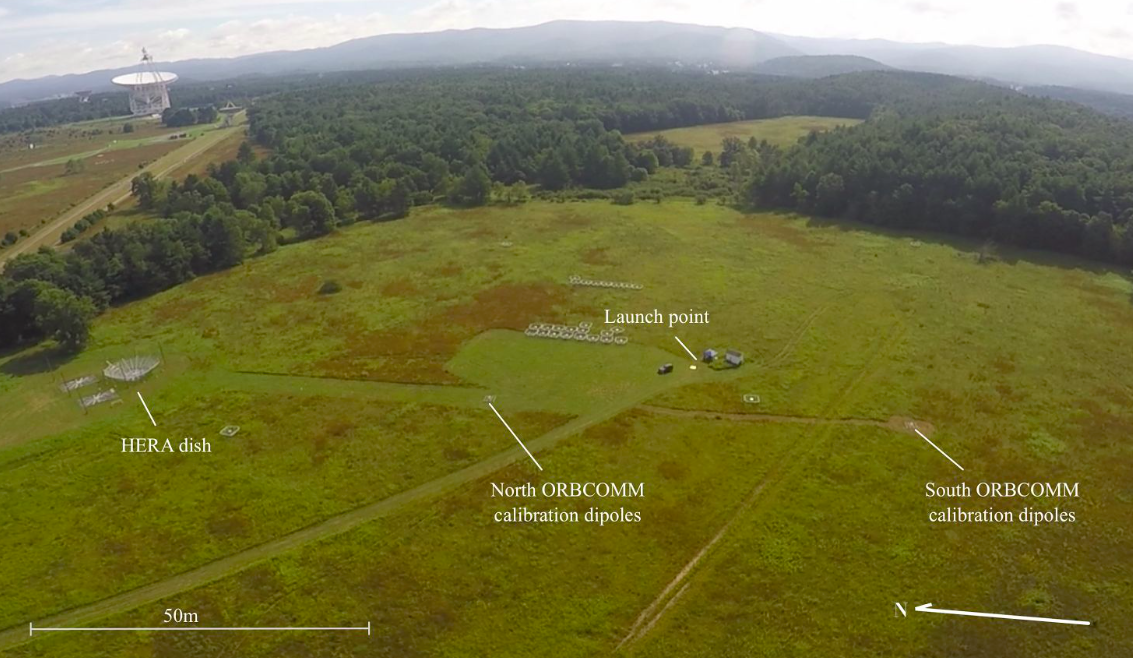
\includegraphics[width=6.5in]{aerial.png}
%\caption{Aerial photograph of the two reference dipoles deployed in Galford Meadow at the National Radio Astronomy Observatory--Green Bank 100\,m south of the HERA dish.}
%\label{fig:aerial}
%\end{figure*}

\subsection{ORBCOMM Beam Mapping System Review}

We briefly review the beam mapping system detailed by \citet{neben15}, then discuss 
application of system to the prototype HERA array at NRAO--Green Bank. The system 
takes advantage of the 137\,MHz communications satellites operated by ORBCOMM Inc. 
as bright point sources which, by virtue of their number ($\sim30$), short orbital periods 
($\sim90$ minutes), and orbital precession cover 65\% of the visible sky in just a few 
days. The coverage is limited by the fact that the satellites' orbital inclinations are all less 
than $45^\circ$. 

In contrast to celestial source beam measurements, though, where the flux may be 
assumed constant over the timescale of the measurement, satellite fluxes can vary rapidly 
due to varying distance, orientation, and transmission power. To correct for this, we 
measure the satellite flux in each ground polarization (EW and NS) using a simple, well-
modeled reference antenna. Comparison of this measured power with that observed in the 
Antenna-Under-Test (AUT) gives the AUT beam response in the direction of the satellite. 
An equivalent interpretation is that the power ratio between the AUT and the reference 
antenna gives the relative beam response in the satellite direction, and multiplication by 
the reference antenna model yields the desired AUT response. As discussed in 
\citet{neben15}, despite the fact that satellite signals are generally polarized, this 
procedure.

In detail, we measure the dual-polarization RMS powers for each antenna in 512 2\,kHz 
bands across the 137--138\,MHz band. Each channel power is averaged over $\sim0.2$
\,sec. There are 0--3 satellites above the horizon at any given time transmitting on different 
$\sim15$\,kHz wide sub-bands in 137--138\,MHz. By observing at many different 
frequencies, we probe the beam response in all these directions simultaneously. We 
compute the satellite positions using the orbital elements published by Celestrak
\footnote{http://www.celestrak.com/NORAD/elements/orbcomm.txt} and the orbital 
integrator \texttt{predict}\footnote{http://www.qsl.net/kd2bd/predict.html}. However, the 
satellite frequencies vary occasionally to avoid interference within the constellation. 
\citet{zheng14} use interferometric phases to identify and exclude times when multiple 
satellites are in view. As our data acquisition system makes only total power 
measurements, we instead use an ORBCOMM interface box (typically supplied to 
commercial users of the network) to sync with passing satellites and record their identifier 
and transmission frequency.

In this way, beam measurements are built up along satellite tracks over the course of 
several days of integration, yielding typically 200--300 satellite pass. Each pass is 
processed separately to identify and exclude times of low signal-to-background when the 
satellite is low in the sky or in the off state of of a pulsing sequence. At those times, then 
satellite flux no longer dominates over that of the diffuse Galactic background, and a 
power measurement no longer probes the response in the satellite direction. The beam 
measurements are then gridded in horizontal coordinates in HEALPix with a resolution of 
$1.8^\circ$ (nside=32). As a last quality control step to reject errant beam measurements 
due to RFI, for instance, we keep only the central 90\% of $\sim50$ measured beam 
values in each HEALPix cell.

%Our power ratio measurement relies upon an accurately modeled reference dipole. We are developing a more comprehensive model of the physical reference antenna and ground screen design, improving on that used in \citep{neben15}. As yet, this improved model yields incorrect results, so more debugging is needed.

\subsection{Assessing Experimental Systematics}

As in \citet{neben15}, we assess systematics using a ``null experiment'' in which we use a second reference dipole as the antenna-under-test (AUT). Taking the ratio of its measured power pattern with the model beam pattern amounts to a ratio of the row power responses received by the two antennas. This test thus probes the level of environmental systematics (i.e., reflections and varying ground properties) and antenna fabrication imperfections which affect each antenna differently. This is not a probe of modeling imperfections common to both antennas, but we expect such errors to be subdominant as the physical properties of the antenna are easier to characterize, and thus simulate, than local environmental effects. 

We run three null experiments with the reference dipoles deployed varying distances from the HERA dish and from each other.

\begin{itemize}
\item \texttt{null1}: reference dipoles deployed 50\,m apart on a NS line, 50\,m south of the HERA dish
\item \texttt{null3}: same as \texttt{null1} but with the south-most reference antenna moved 5\,m west
\item \texttt{null4}: same as \texttt{null1} but with 100\,m separation between both reference antennas and from the dish
\end{itemize}

Figure \ref{fig:null1} shows the results from the \texttt{null1} experiment in the form of the ratio of the power responses of the two antennas (top panel), and slices through the E an H planes of the reconstructed power patterns (bottom panel). We collected roughly 100 satellite passes. Systematics at the few percent level are observed in  within $20^\circ$ of zenith, and at the $\sim10\%$ level farther out.

The magnitude of these systematics is comparable to those observed in the two other null experiments (Figures \ref{fig:null3} and \ref{fig:null4}), an their angular distribution appears largely unchanged. This suggests that the reference dipoles differ both due to varying environmental properties and perhaps intrinsic differences. In any case, these fractional errors propagate directly into the measured beampatterns of our subsequent feed and dish measurements.  

%\begin{figure*}[h]
%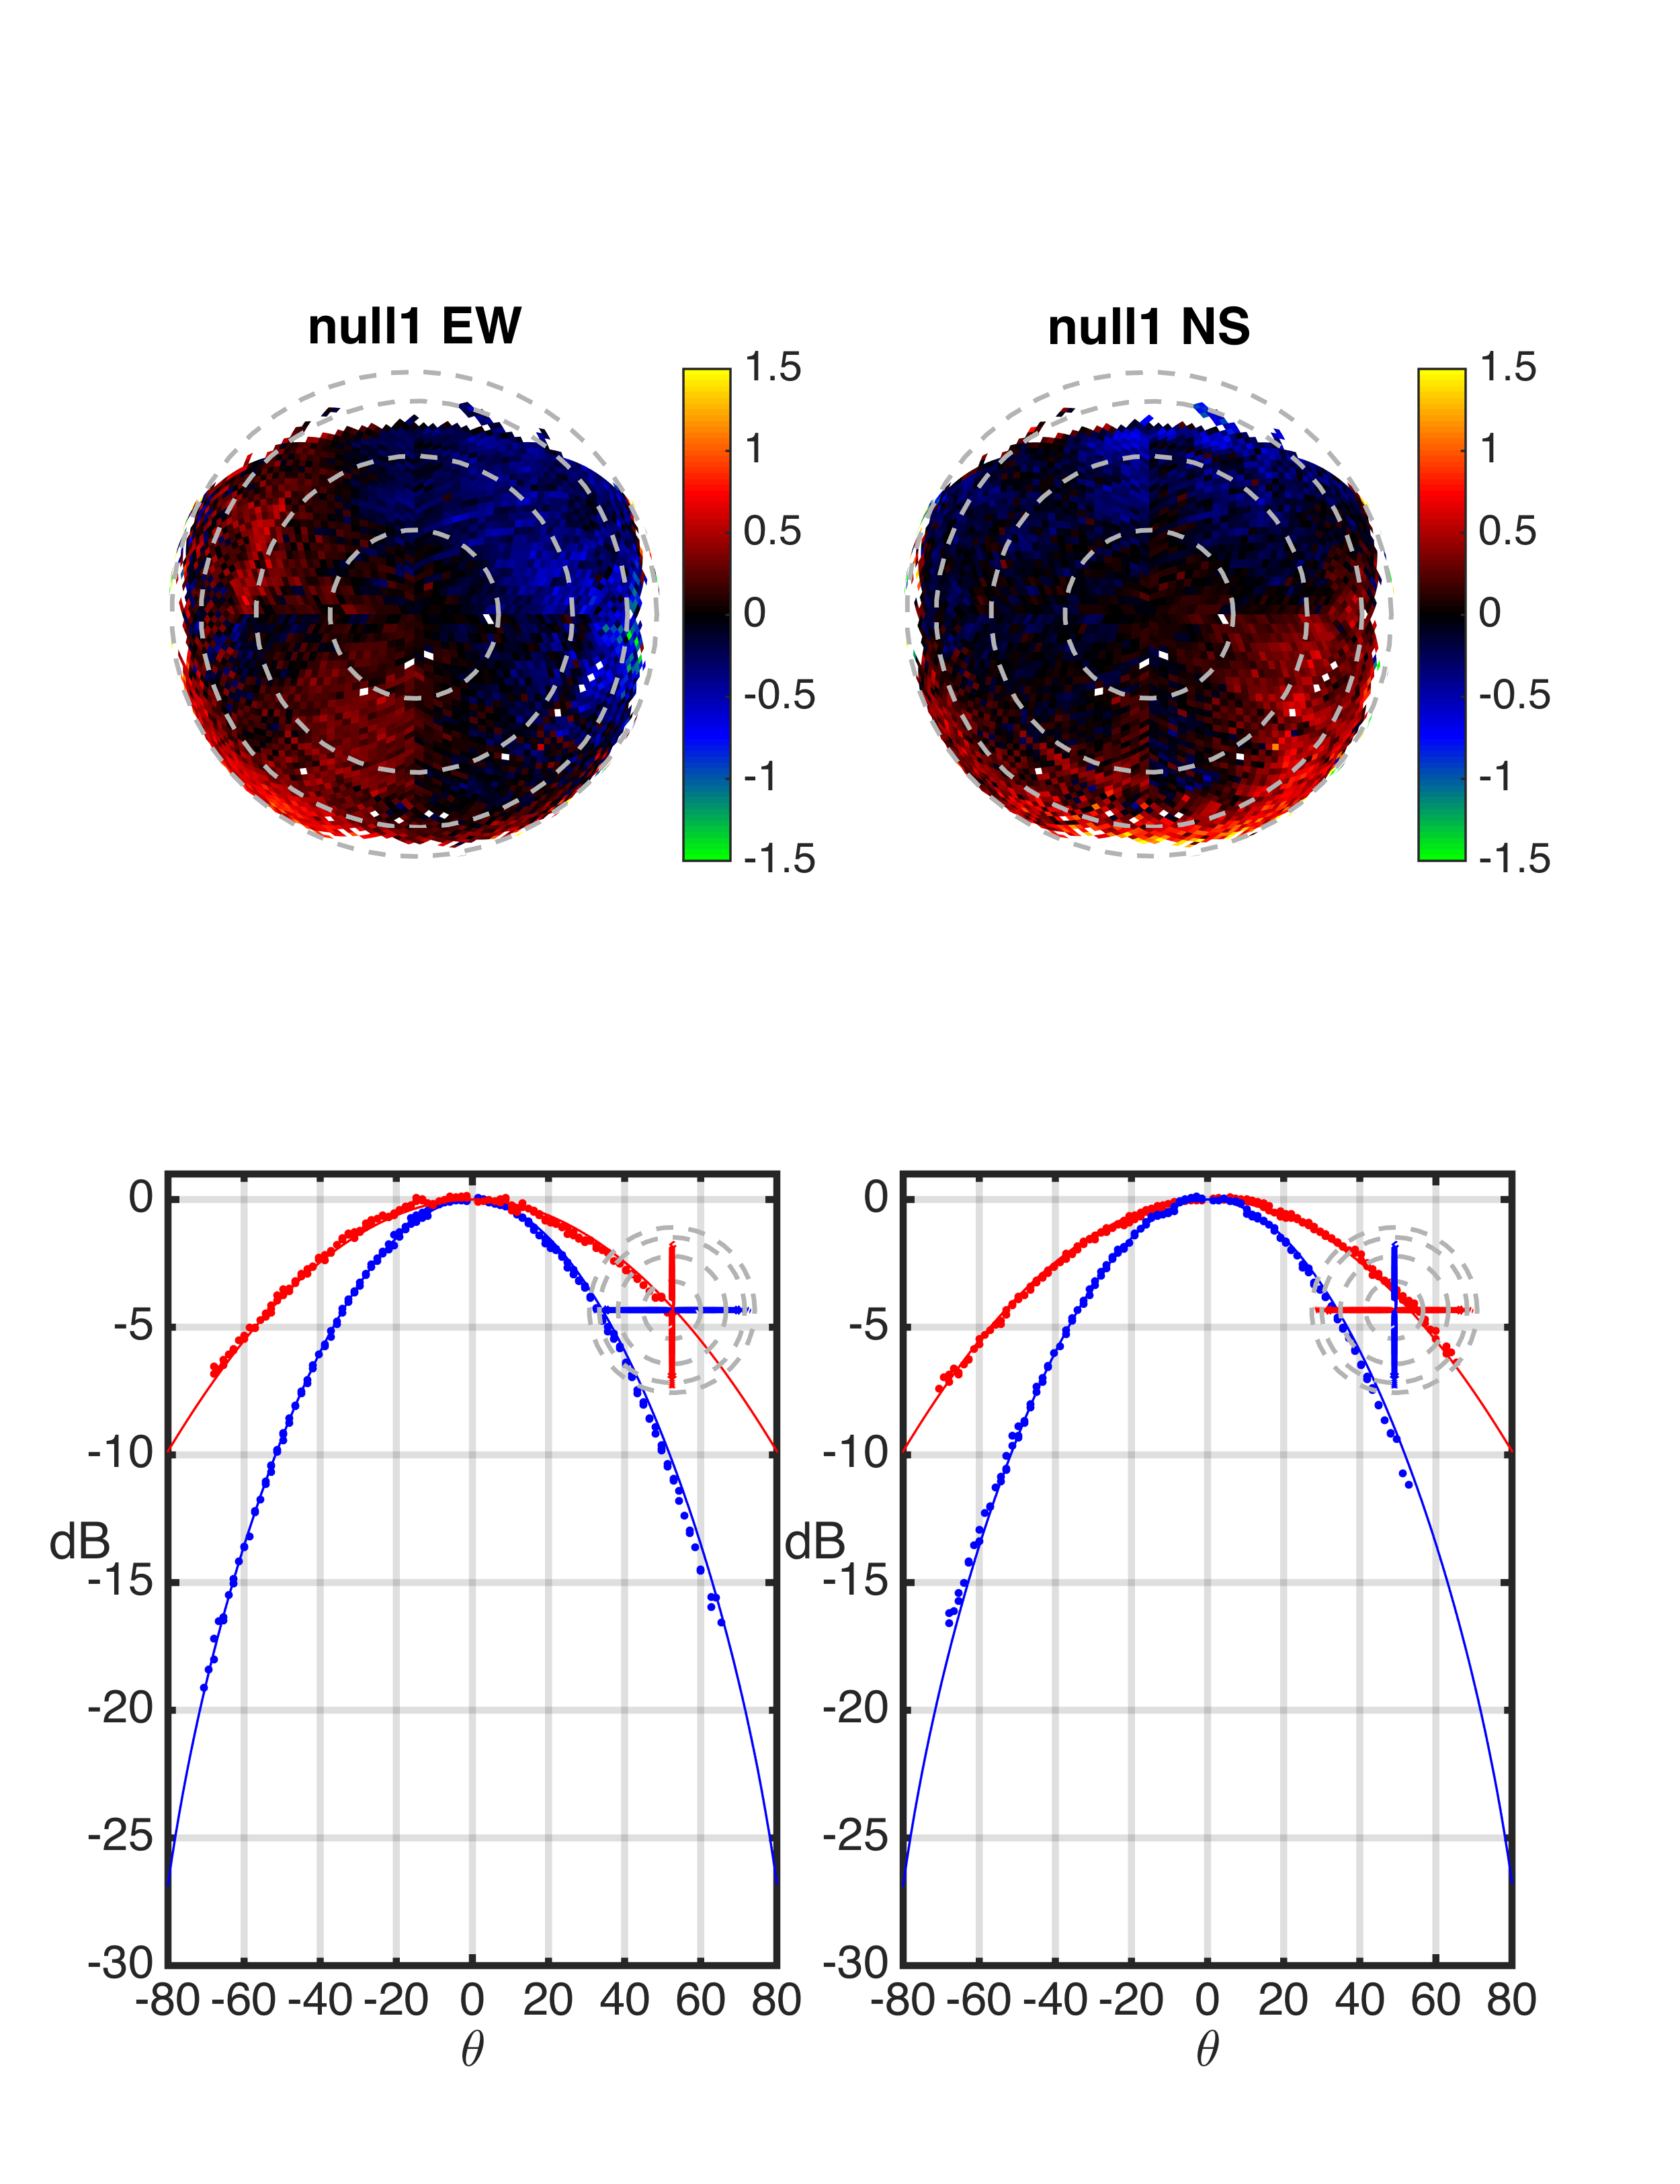
\includegraphics[width=6.5in]{null1_rel.png}
%\caption{Top: ratio maps of the powers received by two reference dipoles separated by 50\,m, deployed 50\,m south of the HERA dish. Bottom: absolute beam power plots constructed by multiplying the relative power maps by a model beampattern. }
%\label{fig:null1}
%\end{figure*}

%\begin{figure*}[h]
%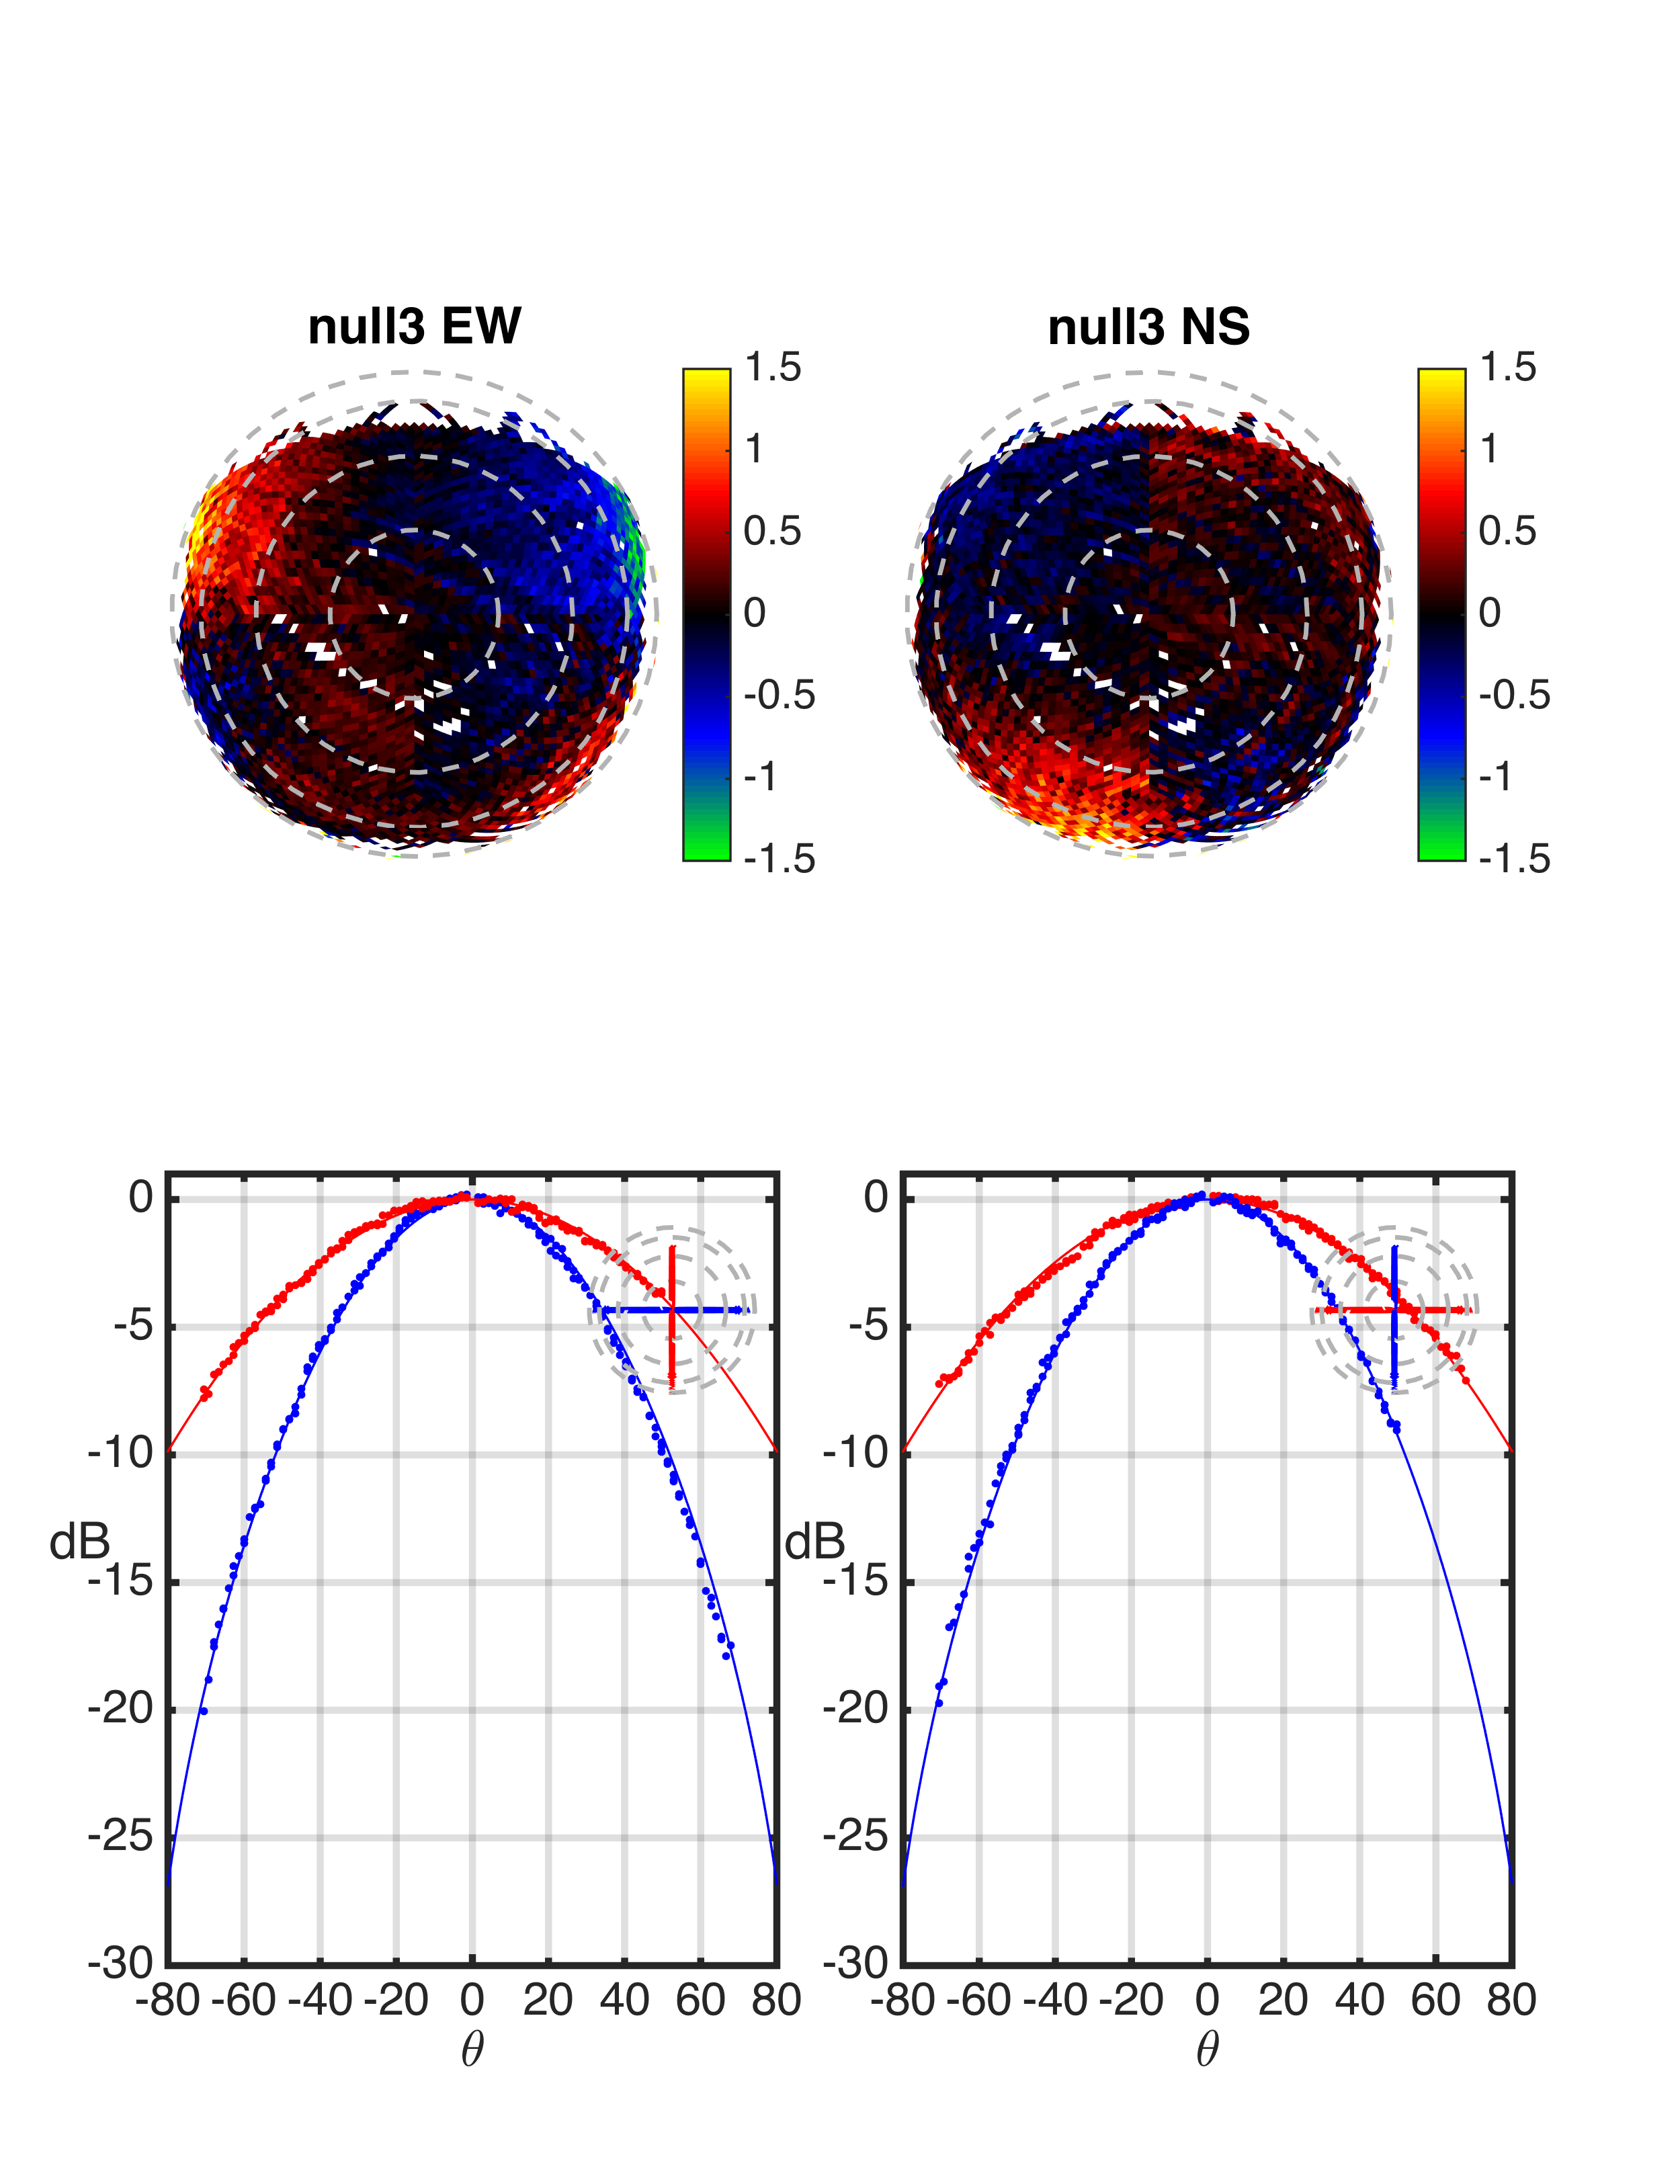
\includegraphics[width=6.5in]{null3_rel.png}
%\caption{Same as the previous null experiment except the south reference dipole was moved 5\,m west. The systematics are largely unchanged.}
%\label{fig:null3}
%\end{figure*}

%\begin{figure*}[h]
%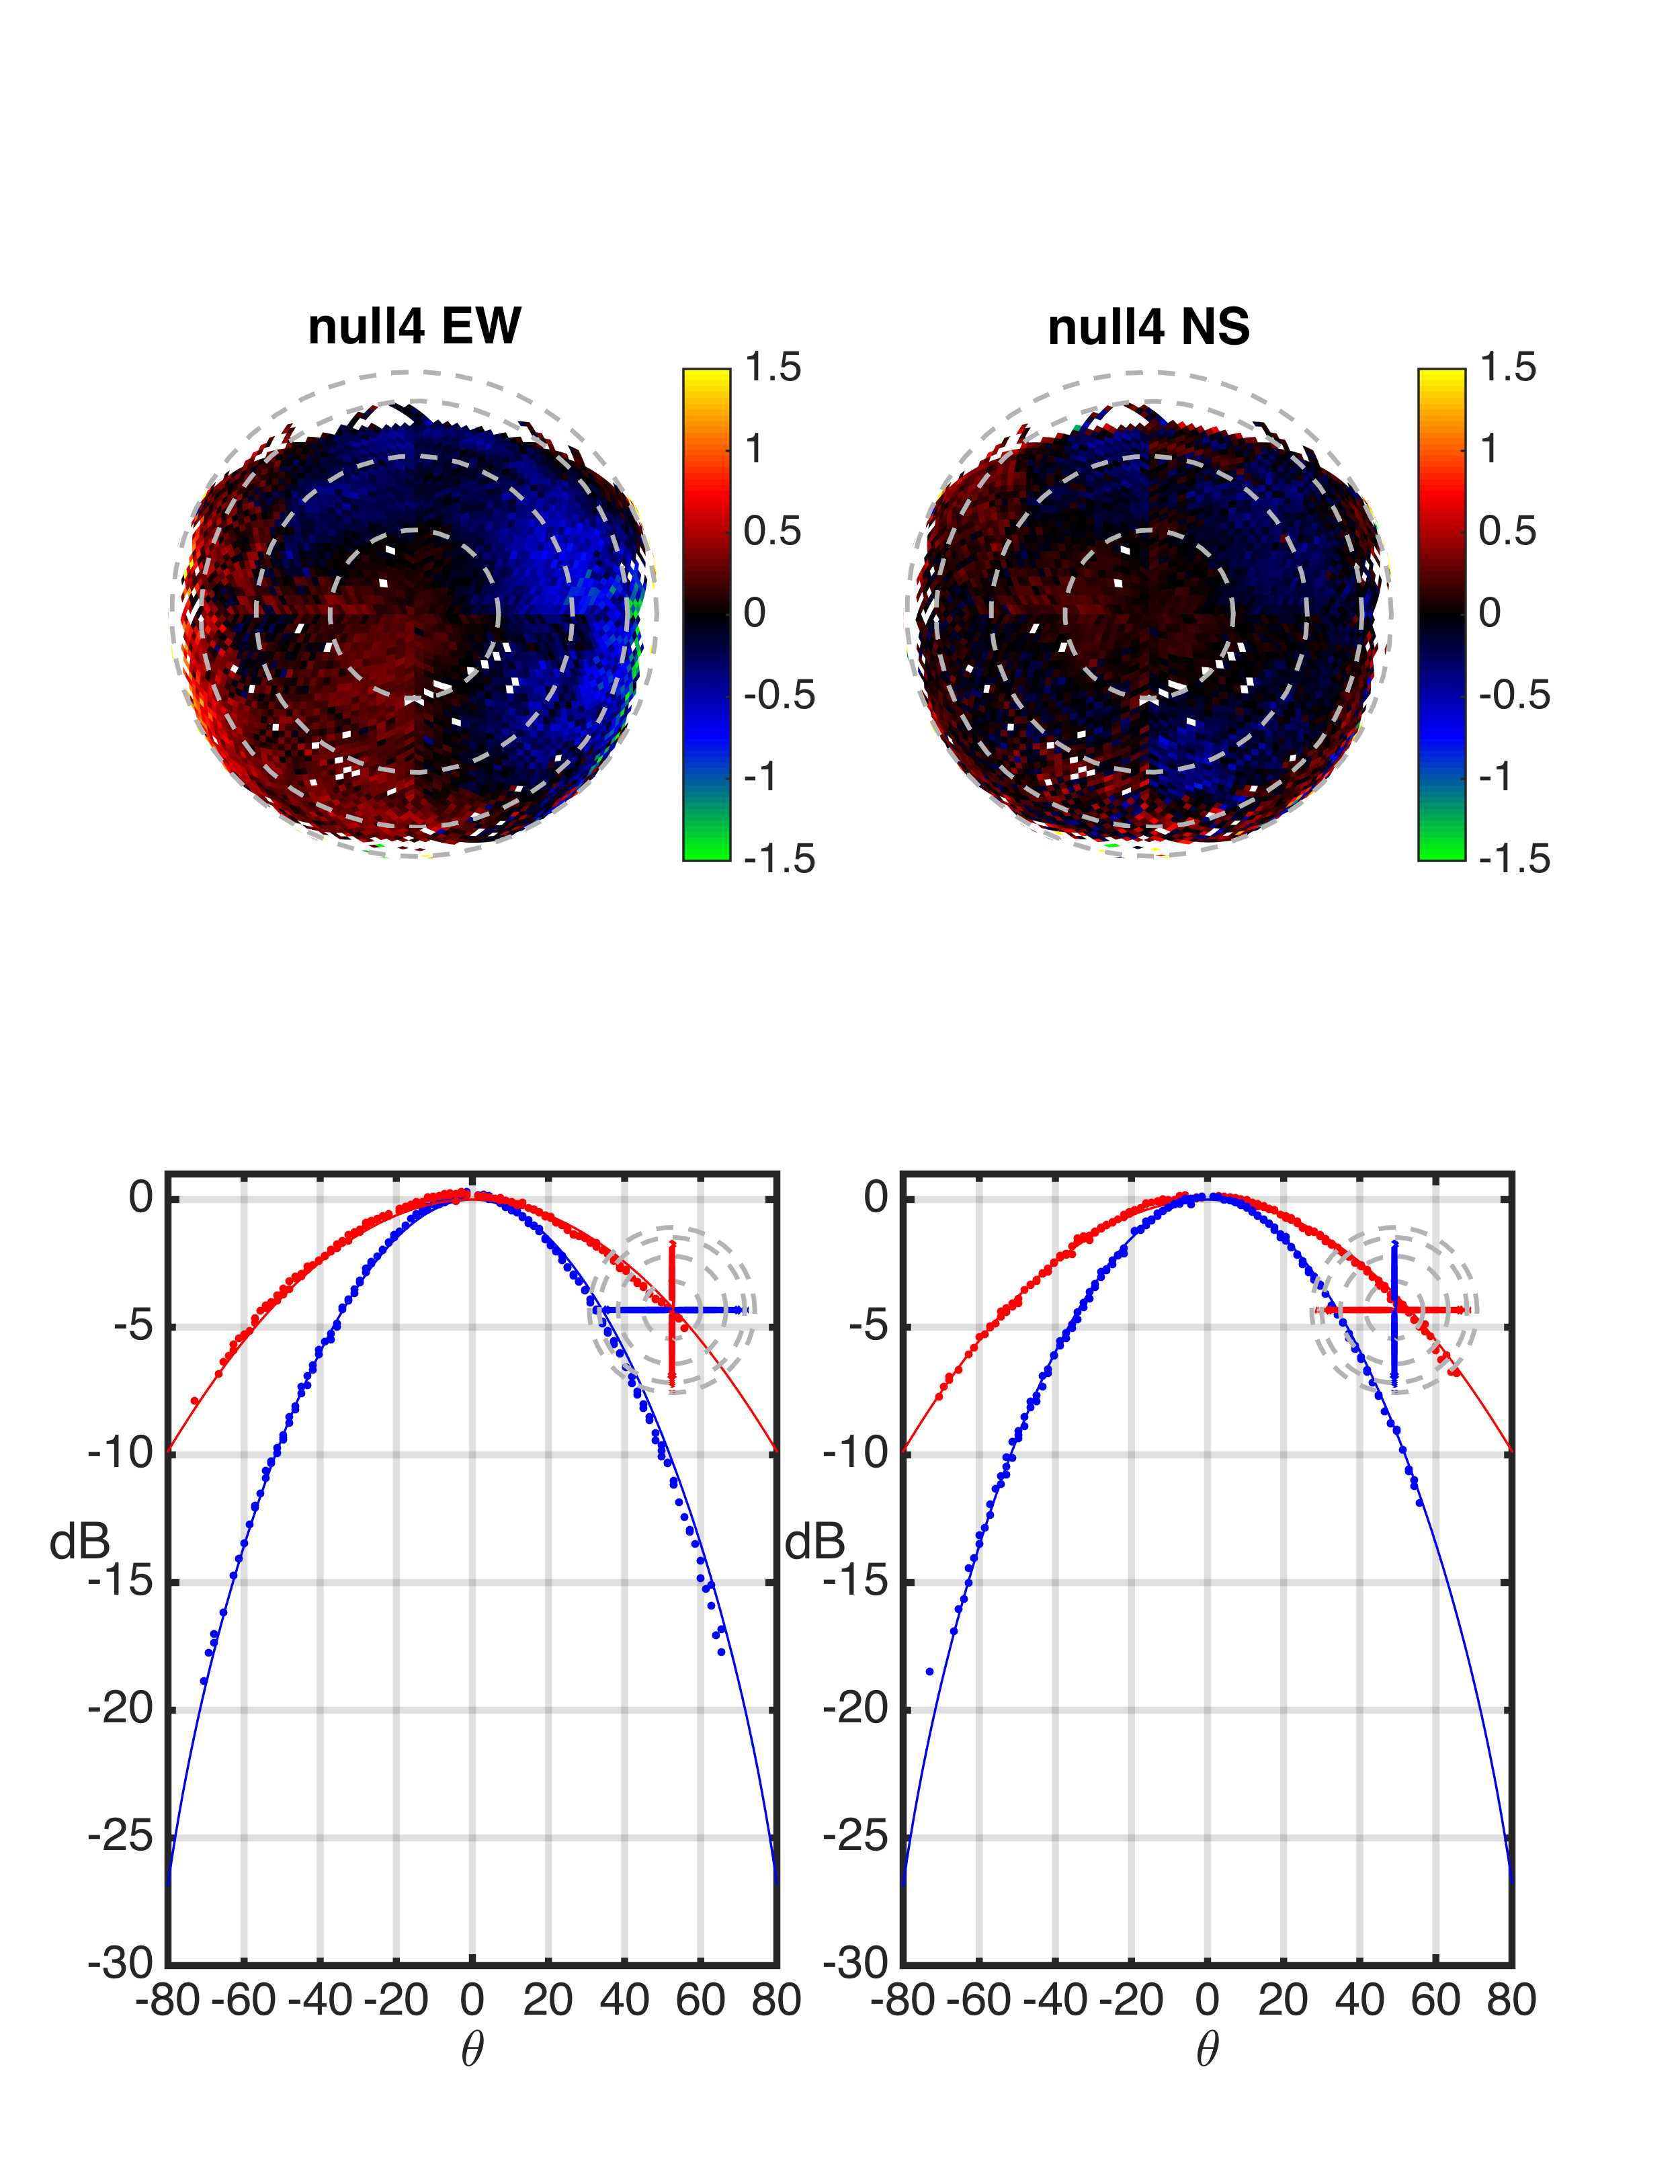
\includegraphics[width=6.5in]{null4_rel.png}
%\caption{Same as the first null experiment except the reference dipoles are separated by 100\,m and deployed 100\,m south of the HERA dish. The systematics remain at the few percent level near zenith and increase to $\sim10\%$ farther out, with somewhat, but not entirely different angular structure. }
%\label{fig:null4}
%\end{figure*}


\section{Dish Measurements}

\subsection{Power pattern measurements}

Having verified the feed power pattern, we deployed feed over the dish and proceed with dish measurements. We measure the power pattern with the feed at four different heights, 4\,m, 4.5\,m, 5\,m, and 5.3\,m, chosen to probe around the nominal focus of 4.5\,m (the nominal beam) and up to the maximum height of 5.3\,m allowed by pole height and rope stresses. Heights are measured from the dish surface to the feed backplane. 

Inspecting the E and H plane slices through the measured beams (bottom panels) in Figures \ref{fig:dish3}, \ref{fig:dish1}, \ref{fig:dish2}, \ref{fig:dish4}, we generally see the main lobe narrow and the sidelobe level decrease. The improvement is also seen in the yellow and red main lobe in the beam maps (top panels) which narrow and approach the expected orientations: the EW (NS) main lobe is elongated in the NS (EW) direction. The last lift produced the smallest change in the beam suggesting it is quite near the best focus. 

The sky coverage in these dish measurements extends out to typically $\theta\sim50-60^\circ$. Beyond that the ORBCOMM flux is sufficiently attenuated relative to diffuse galactic emission that a power ratio measurement between the two antennas is no longer a clean probe of their gains in the direction of the satellite. At these zenith angles, the beam sidelobes are roughly -30\,dB, and seem to be trending downward at the edge of the measured region.

%\begin{figure*}[h]
%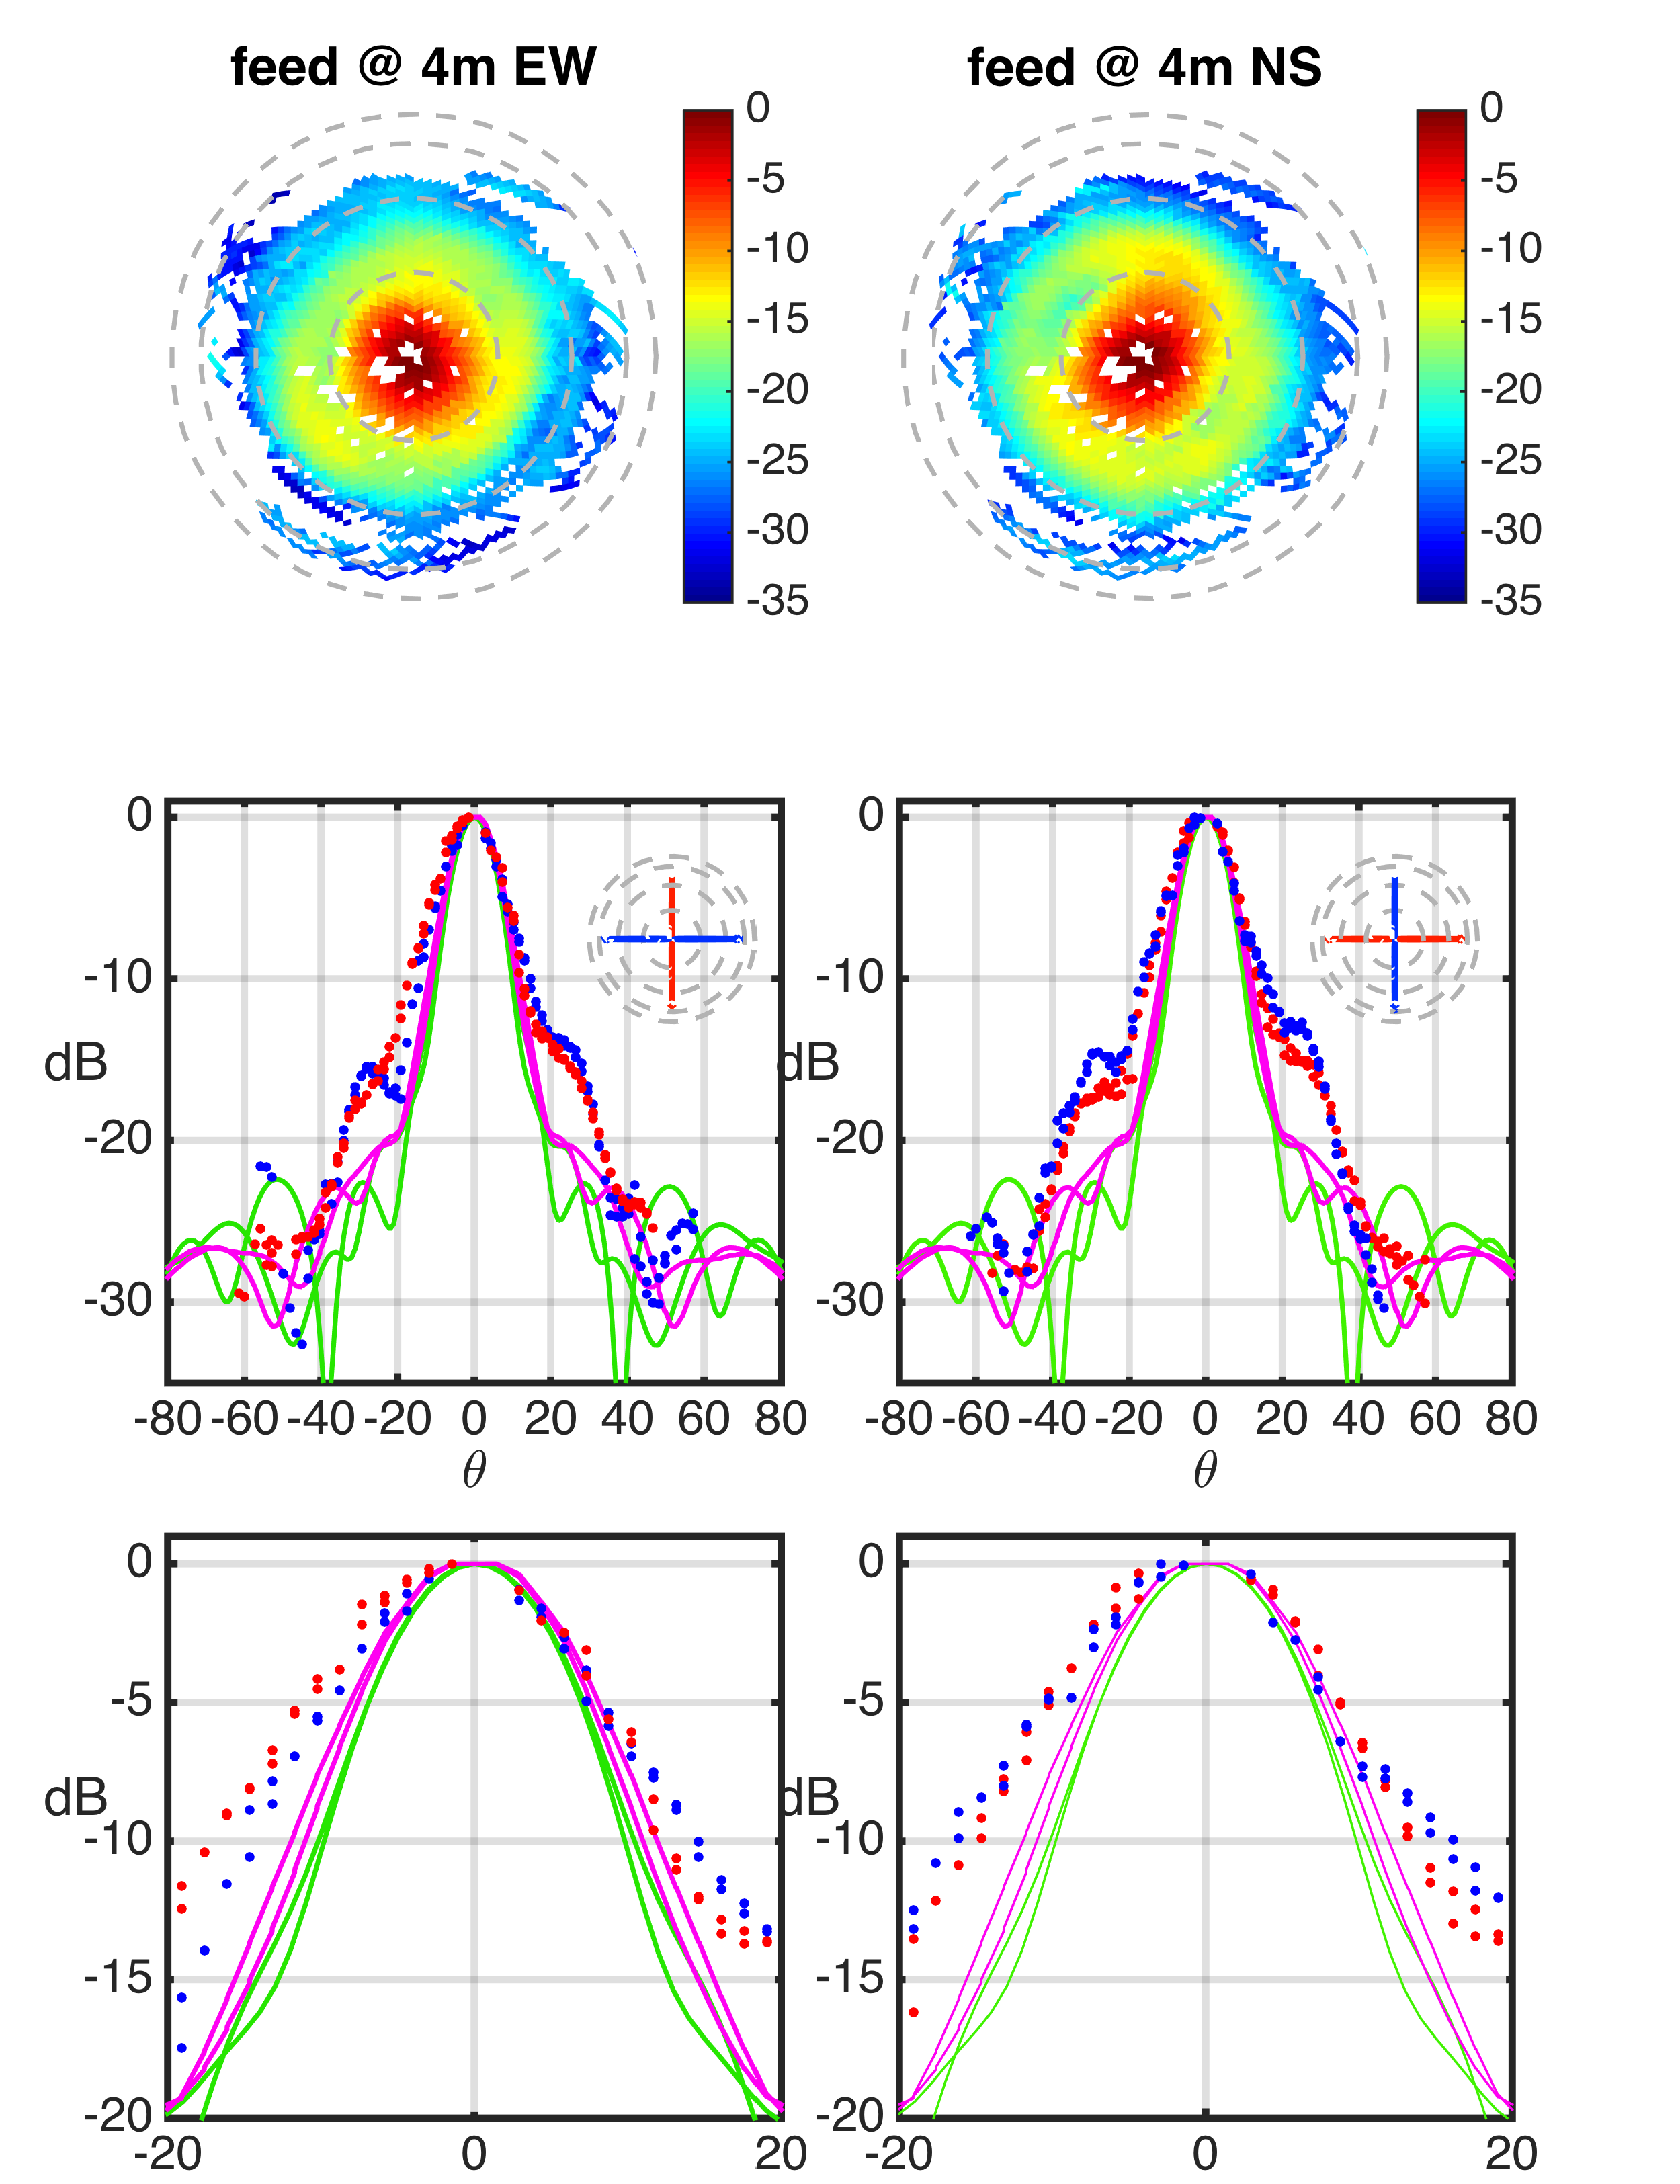
\includegraphics[width=6.5in]{dish3_abs_old_ref_model.png}
%\caption{Dish power pattern with the feed lowered 0.5\,m below nominal focus.}
%\label{fig:dish3}
%\end{figure*}

%\begin{figure*}[h]
%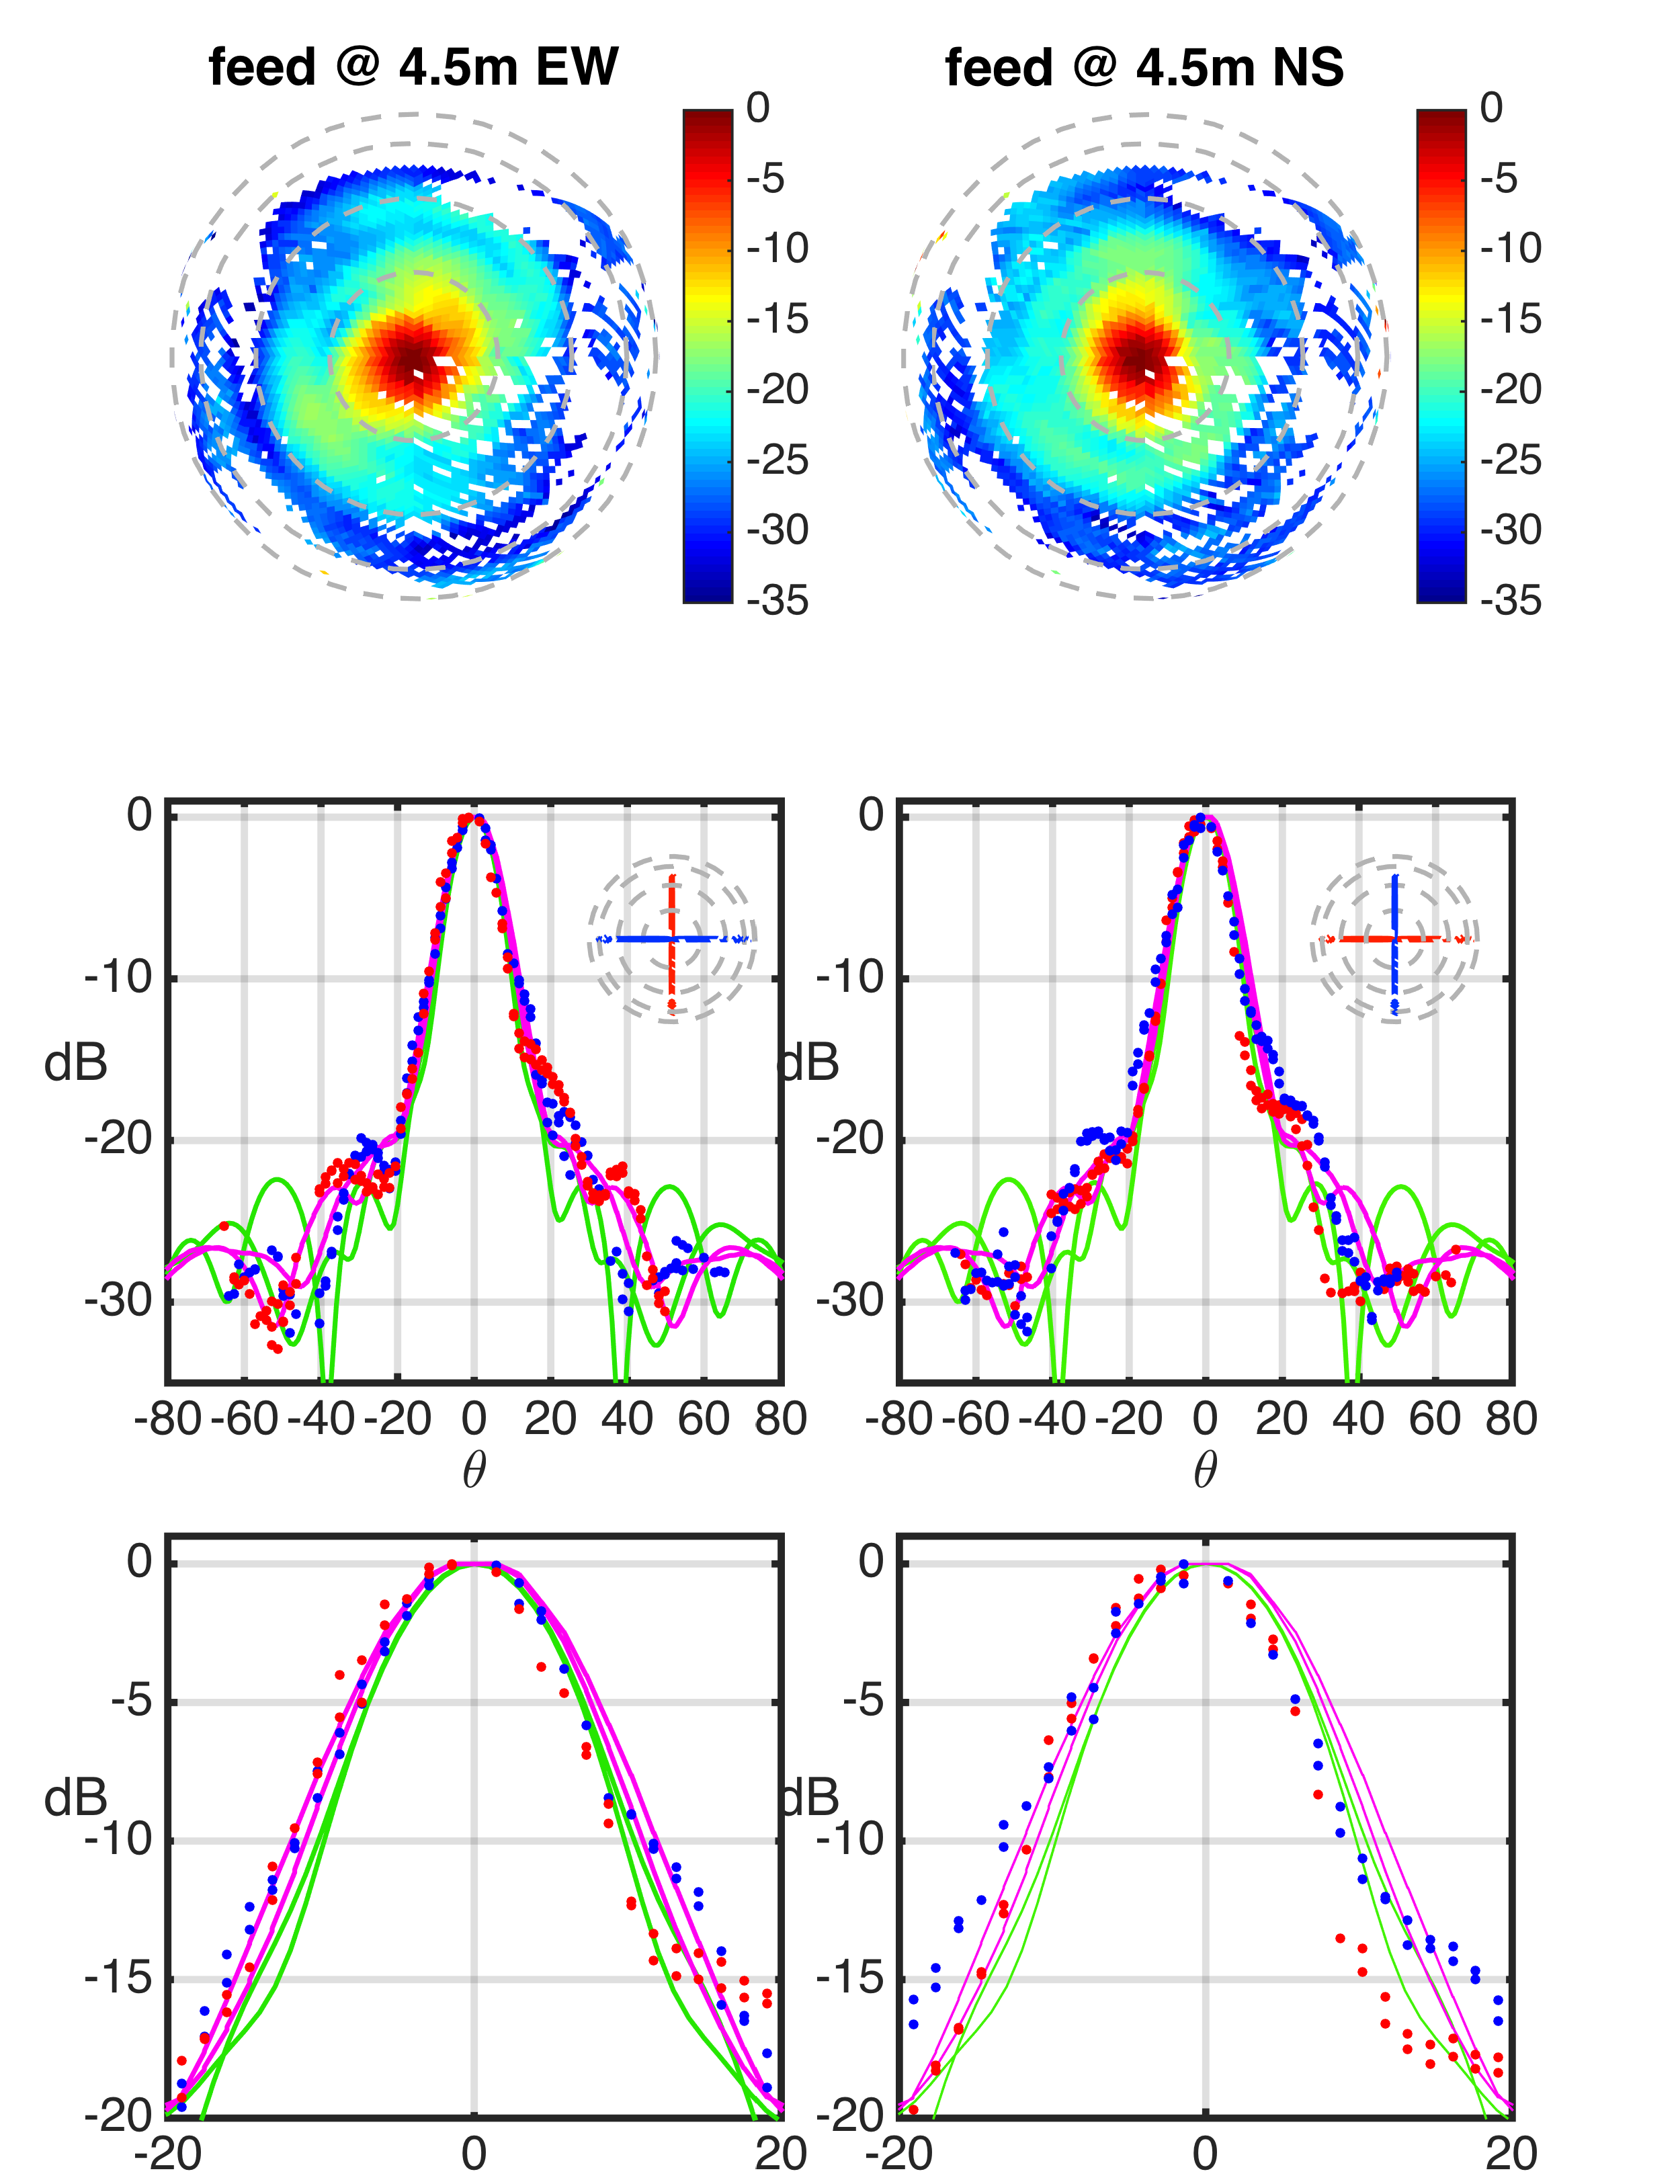
\includegraphics[width=6.5in]{dish1_abs_old_ref_model.png}
%\caption{Dish power pattern with the feed at the nominal focus of 4.5\,m.}
%\label{fig:dish1}
%\end{figure*}

%\begin{figure*}[h]
%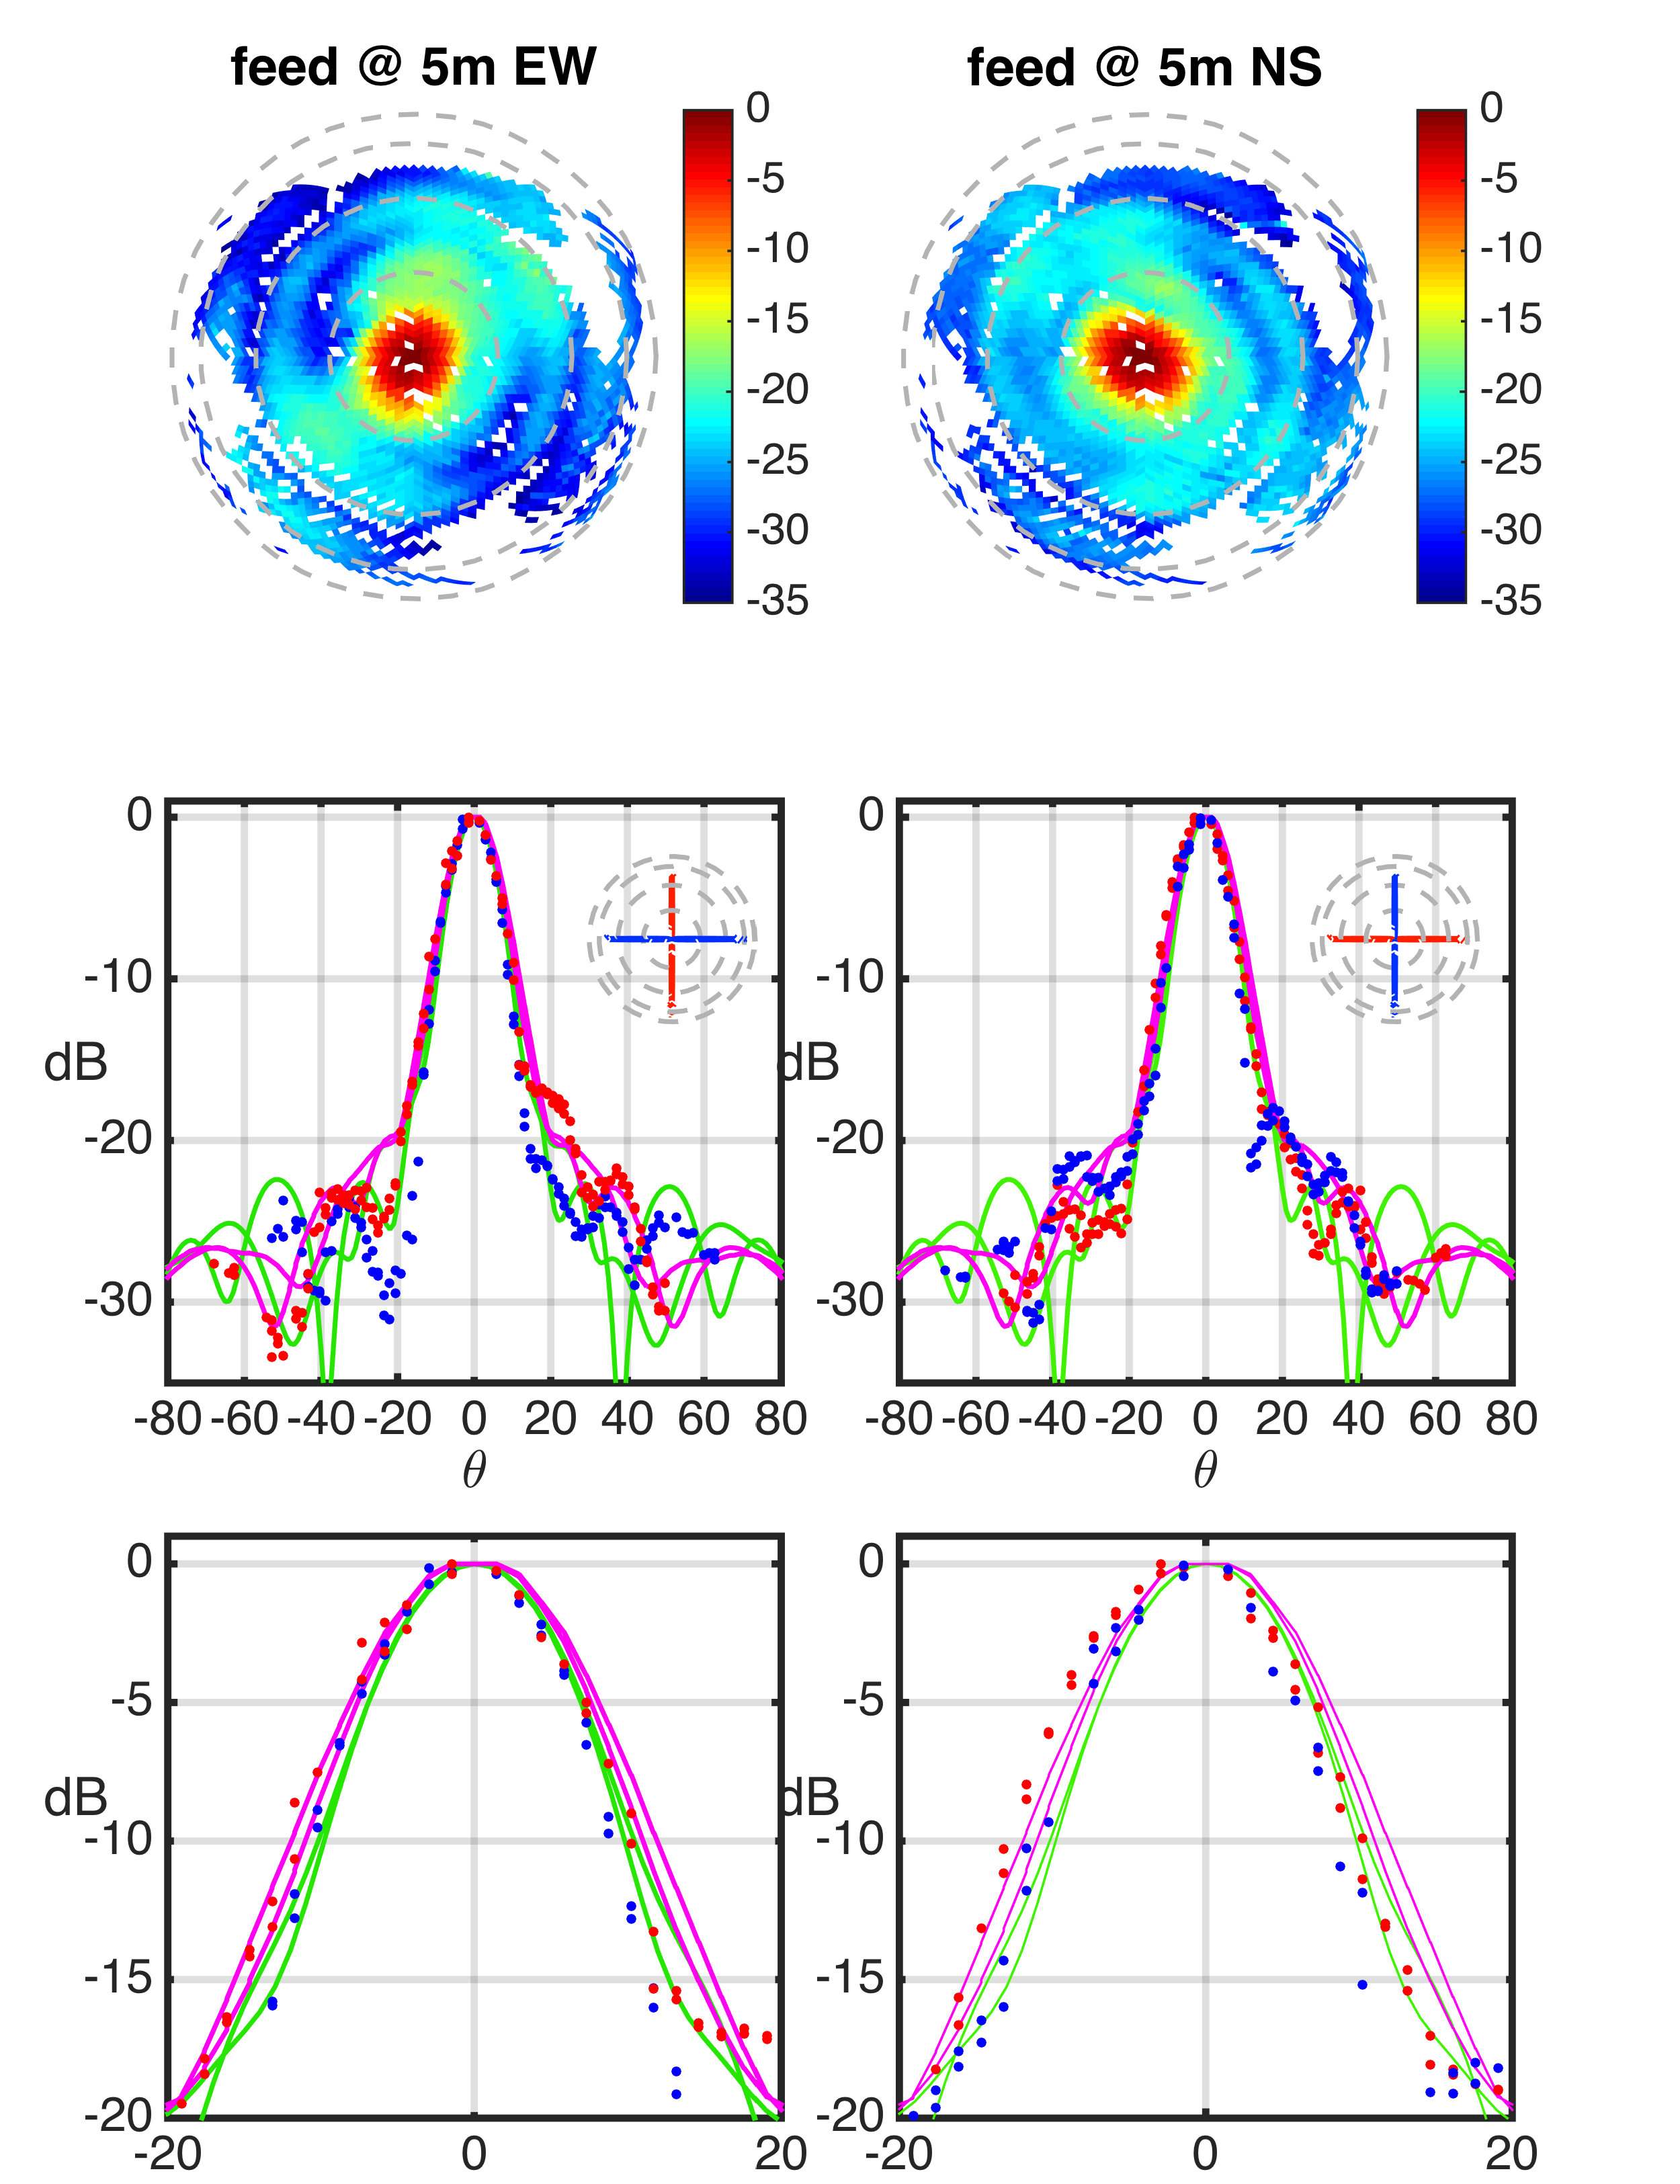
\includegraphics[width=6.5in]{dish2_abs_old_ref_model.png}
%\caption{Dish power pattern with the feed raised 0.5\,m above nominal focus.}
%\label{fig:dish2}
%\end{figure*}

%\begin{figure*}[h]
%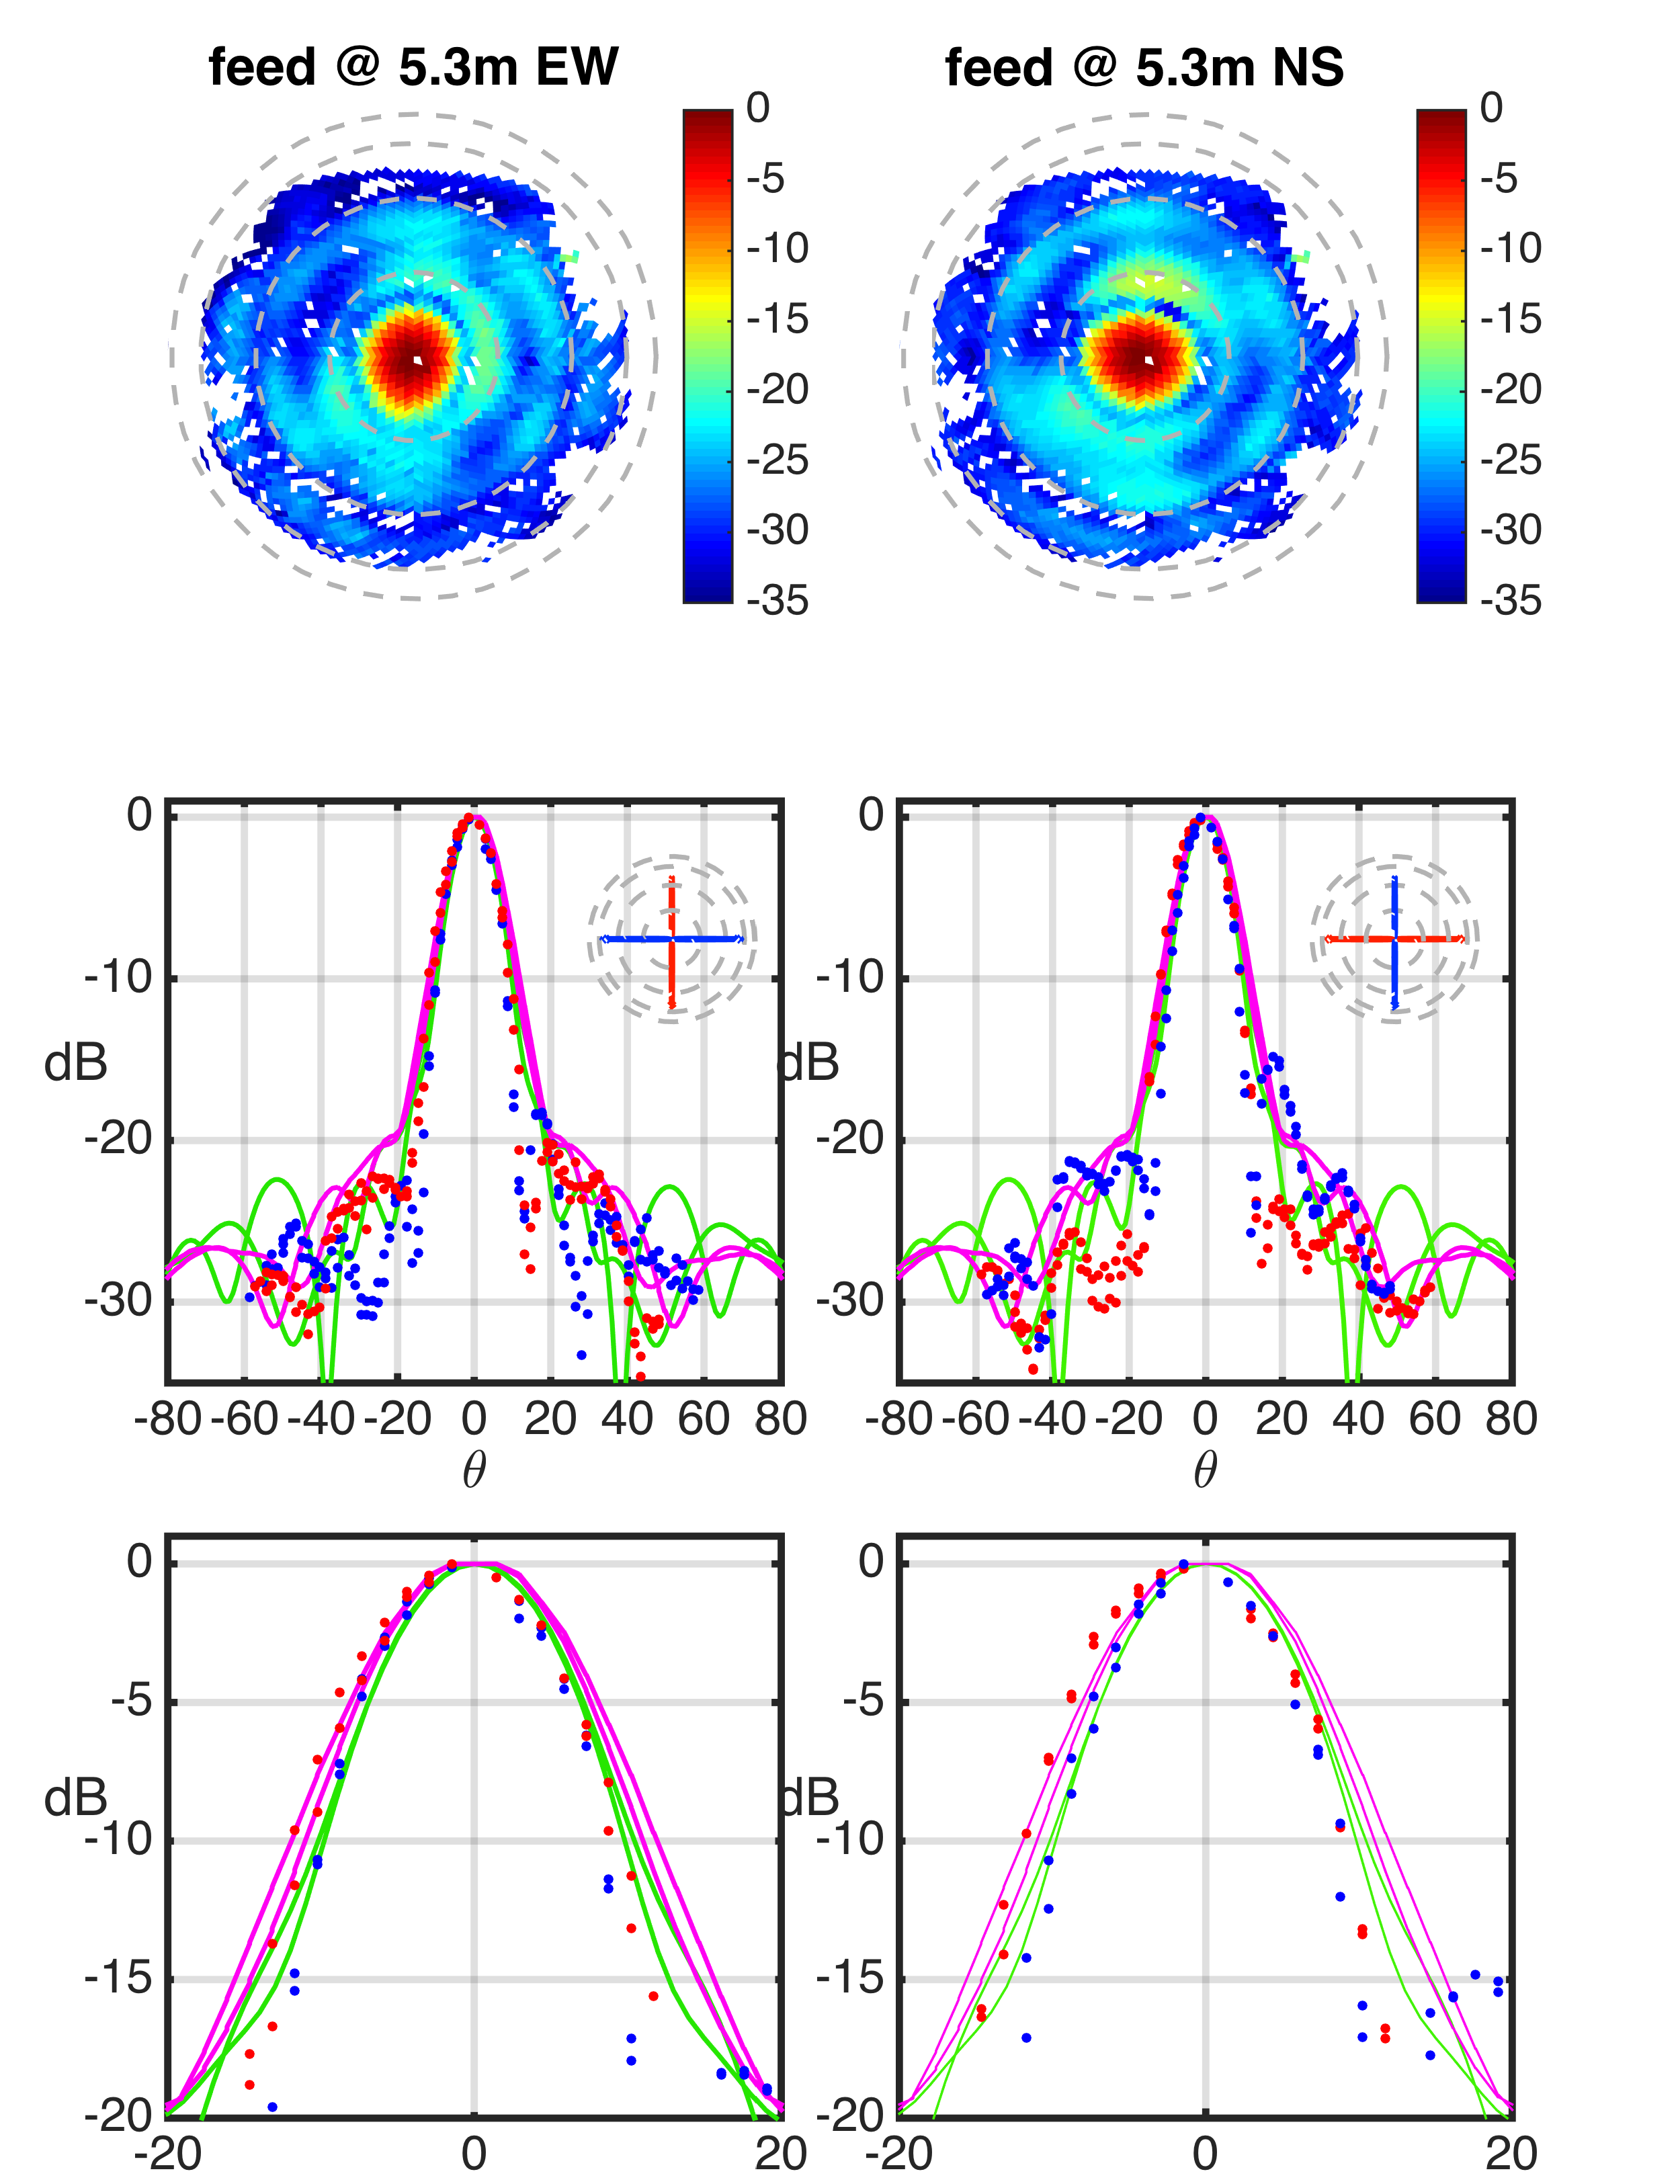
\includegraphics[width=6.5in]{dish4_abs_old_ref_model.png}
%\caption{Dish power pattern with the feed raised to its maximum height of 0.8\,m above nominal focus.}
%\label{fig:dish4}
%\end{figure*}

In order to compute beam collecting areas and assess foreground leakage we require a beam covering the entire visible sky. For each measured dish beam, we interpolate over the unmeasured cells at $\theta\lesssim60$, then extrapolate outward to the horizon. This amounts to a smooth continuation of the beam response at the same $\sim-30$\,dB level suggested by the fringes of our measurements. We take this as a first possible model of the full sky dish beam, and construct a second with a gaussian cutoff at $\theta=60^\circ$ with $\sigma=2.5^\circ$, the pair of which span the space of likely horizon responses. This procedure is depicted in Figure \ref{fig:interpbeams} where we plot the measured nominal focus beam, the beam after interpolation and extrapolation, and the beam after applying the gaussian cutoff. Figure \ref{fig:interpbeamsslice} shows the interpolated/extrapolated beam and the beam with the cutoff along with various models to illustrate the different horizon responses more clearly.

%\begin{figure}[h]
%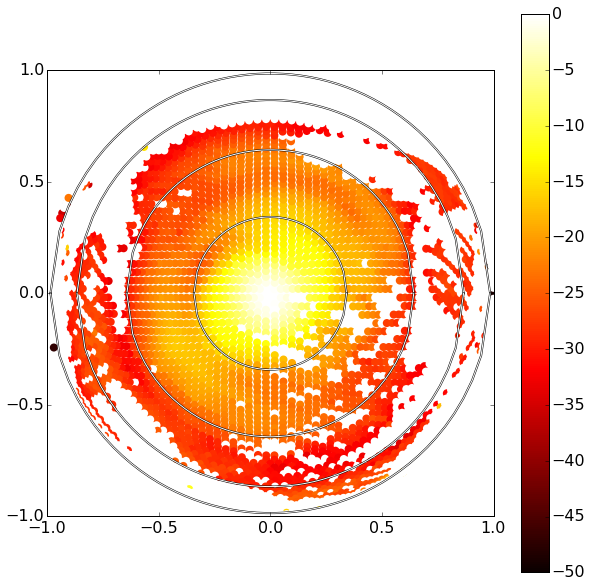
\includegraphics[width=3.5in]{measbeam_raw.png}
%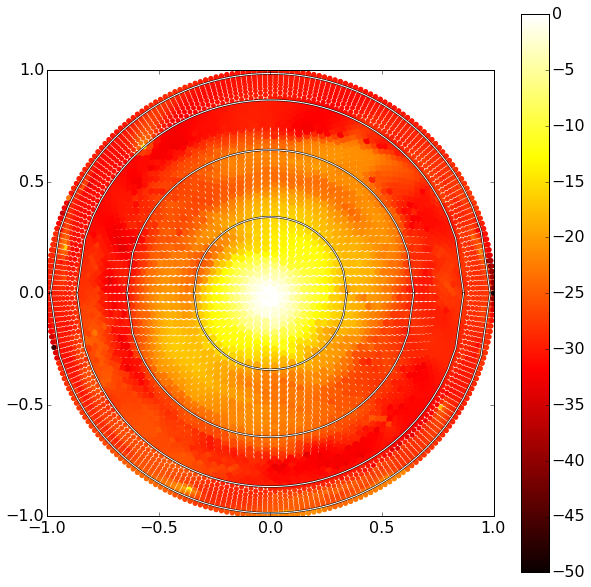
\includegraphics[width=3.5in]{measbeam_interp.png}
%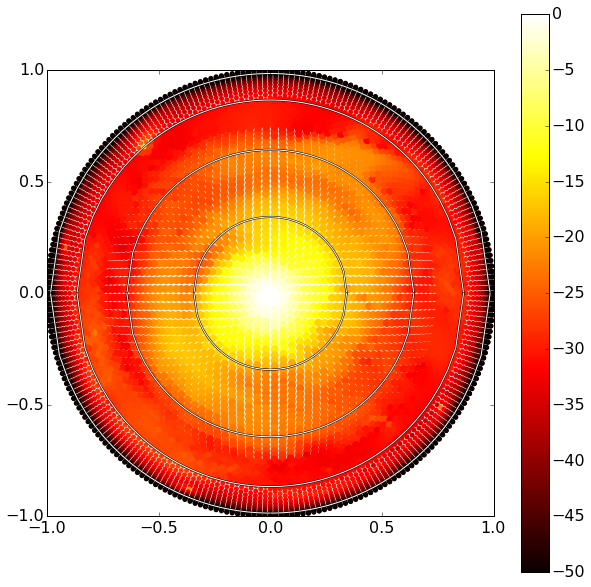
\includegraphics[width=3.5in]{measbeam_interp_expcutoff.png}
%\caption{We construct full sky beams as required for Section \ref{sec:foregroundleakage} by starting from the nominal focus beam (top left), interpolating over unobserved cells at $\theta\lesssim60^\circ$ and extrapolating to the horizon (top right), and applying a gaussian cutoff starting at $\theta=60^\circ$ with $\sigma=2.5^\circ$ (bottom left). These last two beams span the space of likely horizon responses. Circles denote $\theta=20^\circ,40^\circ,60^\circ,80^\circ$.}
%\label{fig:interpbeams}
%\end{figure}

%\begin{figure}[h]
%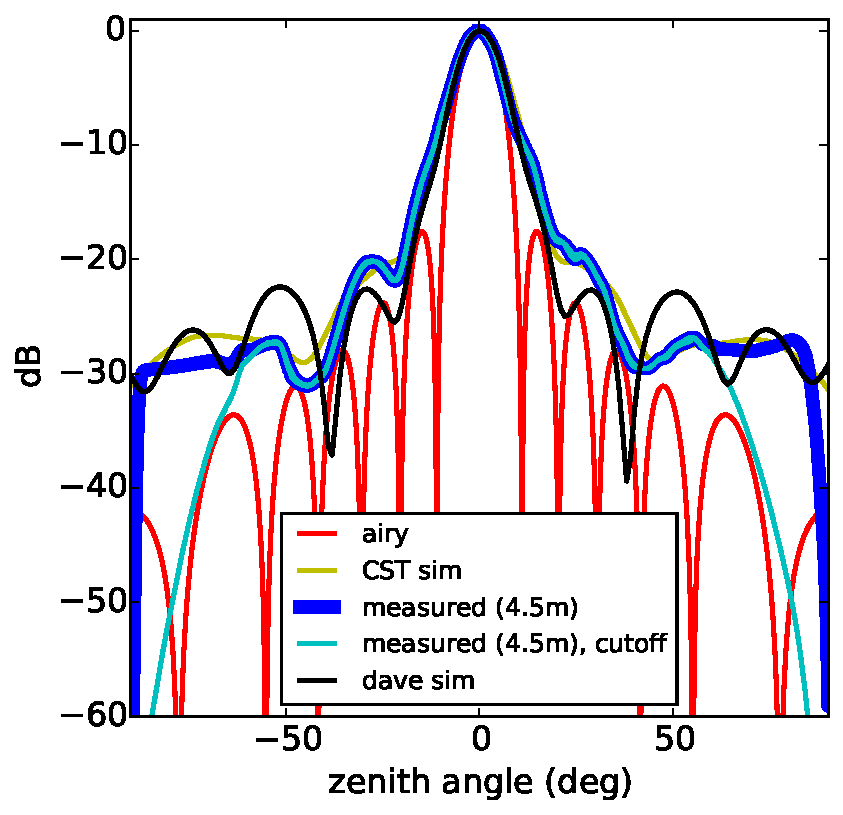
\includegraphics[width=3.5in]{ew_beams_slice.pdf}
%\caption{We plot the interpolated/extrapolated measured nominal focus  beam itself (blue), and with the gaussian cutoff (cyan), along with various model beams to illustrate the varying horizon responses. }
%\label{fig:interpbeamsslice}
%\end{figure}

To illustrate the results of these smoothing operations we plot slices through the nominal focus dish beam along with the three model beams discussed in Sec. \ref{sec:dishmodels}. The H (E) plane slice of the main lobe is shown at the top (bottom). The plots in the left side zoom in on the main lobe, while those on the right show a zoomed out view of the entire sky pattern. 

\subsection{Collecting Area}

The collecting area of the antenna is related to the power pattern by the ratio of the beam gain to its beam-weighted solid angle as
\begin{equation}
	A=\frac{\lambda^2 B(0,0)}{\int B(\theta,\phi)d\Omega}
\end{equation}
We evaluate the collecting area for four of the beams discussed above and present the numbers in Table 1. We are unable to quantify the collecting area of the beam from Dave's simulation because it was run at too coarse an angular resolution. For the measured beams, we compute the collecting area using the interpolated/extrapolated beams with and without the gaussian cutoff at $\theta=60^\circ$.

 \begin{table}[h]
 \caption{ \label{table:collectingareatable}Collecting area (m$^2$) for modeled and measured dish beams at 137\,MHz. For measured beams, we calculate the collecting area after interpolation/extrapolation, also with the $60^\circ$ gaussian cutoff (in parentheses).}
\begin{tabular}{| l | l | l |}
\hline
  Airy & 155\,  \\
  CST sim & 67.0\,  \\
  \hline
  Measured, feed at 4\,m & 42.1 (44.3) \\
  Measured, feed at 4.5\,m & 68.5 (73.6) \\ 
  Measured, feed at 5\,m & 77.1 (82.6) \\
  Measured, feed at 5.3\,m & 93.0 (97.9)\\
  \hline
\end{tabular}
\end{table}

By definition, the Airy pattern has the largest collecting area equal to the dish cross section. The others model a realistic feed with a hanging screen (the skirt or ``kilt''), effectively tapering the dish response to radiation received from its fringes to mitigate cross-coupling and crosstalk between adjacent dishes. As expected, raising the height of the feed increases the illuminated area of the dish, and thus, its collecting area. As expected, the measured collecting area matches that of the CST model at the nominal focus height of 4.5\,m.

Why does the collecting area increase as the feed is raised over the nominal focus? There are two computing effects here: (1) the reflected radiation is less well focused above the feed, decreasing the response; and (2) the tapered feed sees a larger dish as it is raised, allowing more radiation to reach the dipole as opposed to reflecting off the skirt. These data suggest that the second effect wins. Of course the reason for the skirt is to taper the feed beam in order to mitigate cross-talk and cross-coupling between the dishes. A larger collecting area may not be worth it in exchange for exacerbating these concerns.

\section{Foreground Leakage and Residuals}
\label{sec:foregroundleakage}

We assess the level of foreground leakage into the EOR window due to beam shape, baseline length, and LST. In particular, we built on the study of \citet{nithya15} of the impact of beam shape and horizon response on foreground spectral structure and containment in the wedge.

We simulate delay spectra for several model and measured beams on different baseline lengths for different LSTs and baseline orientations. All these factors affect the level of emission horizon brightening in delay space, the ``pitchfork'' effect, and the level of foreground leakage. We assume a constant beam pattern over that band, with leakage due only to the finite bandwidth and choice of window function. Actual frequency structure imprinted onto the foregrounds by variation of the beam angular pattern or overall gain with frequency (Patra et al.)

We begin by simulating visibilities over a 20\,MHz bandwidth with  400\,kHz resolution centered on 137\,MHz on two different baselines for two model beams (airy, and CST sim) and two measured beams (measured nominal focus beam, and measured nominal focus beam with $60^\circ$ cutoff). We use the short and maximally redundant 14\,m baseline, most useful for delay spectrum analysis, as well as a longer 42\,m baseline, more useful for imaging analysis. From these frequency-sequenced visibilities we calculate the delay spectrum  \citep{perbaselinetechnique} using the Blackman-Harris window following \citet{nithya15}. This window reduces the noise equivalent bandwidth to 10\,MHz, corresponding to $\Delta z\sim0.5$, beyond which evolution of the cosmological signal become significant. Larger bandwidths, though, are useful for foreground estimation and delay-space deconvolution \citep{parsonsandbacker,paper32,paper64}. With this caveat, our simulated delay spectra show the worst case scenario, quantifying the level of foreground isolation without estimation and deconvolution.

Our sky model is comprised of a deep MWA point source survey within 20$^\circ$ of R.A.(J2000) $= 0^\text{h}\,0^\text{m}\,0^\text{s}$ and decl.(J2000) $= -30^\circ\,0'\,0''$ (Carroll et al., in prep.), the shallower but wider MWA commissioning point source survey\citep{MWACS}, the Culgoora catalog\citep{Slee1995}, and the Global Sky Model of Galactic radio emission \citep{gsm}. 

Figure \ref{fig:delayspec} shows the delay spectra at $0^\circ$ (top pair) and $60^\circ$ (bottom pair) LST for 14\,m (left pair) and 42\,m (right pair) EW baselines. For reference we plot a 1D model 21\,m power spectrum for $z\sim8$ from \citet{21cmfast}. Consider first the $0^\circ$ LST plots where the Galactic disk has nearly, but not completely set. The effect of horizon response is most visible on the longer 42\,m baseline where the measured beam (red) and CST model (yellow), both show significant brightening at the horizon delays (vertical black lines) due to roughly -30\,dB beam response near the horizon, as discussed by \citet{nithya15,nithya15}. In contrast, the airy model (black) and measured beam with cutoff (blue) show no significant brightening at the horizon, where they appear still to be dominated by the wings of the delay PSF from the emission closer to zero delay. 

We also plot (green dashed line) the delay spectrum after subtracting the visibilities computed with the $\theta\sim60^\circ$ cutoff measured beam from those using the full measured beam. This curve may be interpreted as the uncertainty in the ``pitchfork'' horizon brightening due to uncertainty in the beam horizon response, or equivalently as the delay spectrum residual foregrounds after subtracting foregrounds in the well modeled region of the sky (Neben et al. 2015b, submitted). By construction, this subtraction leaves emission from the highest delay regions of the sky (near the horizon on opposite sides of the baseline), but also leaves some low delay emission on opposite sides of a line perpendicular to the baseline. However, this additional low delay emission near the horizon gets drowned out by that from near zenith where the beam is substantially stronger. 

On the shorter 14\,m baseline, the horizon brightening is smaller because there is roughly an order of magnitude more emission at zero delay, whose thereby stronger delay wings, which are also relatively wider compared to the narrower foreground wedge, cover up much of the edge brightening. At $60^\circ$ LST, effect of horizon response is much smaller as the Galactic disk is now entirely below the horizon. 

The level of leakage depends also on baseline orientation which sets which directions on the sky map to large delays. Figure \ref{fig:delayspec2} shows the delay spectra at $0^\circ$ LST on 14\,m NE (top pair) and SE (bottom pair) baselines. Both show increased edge brightening compared to the 14\,m EW baseline. \citet{nithya15} proposes to identify through modeling the baselines most susceptible to this edge brightening at any given time, and simply exclude them from the power spectrum analysis. 



%\begin{figure*}[h]
%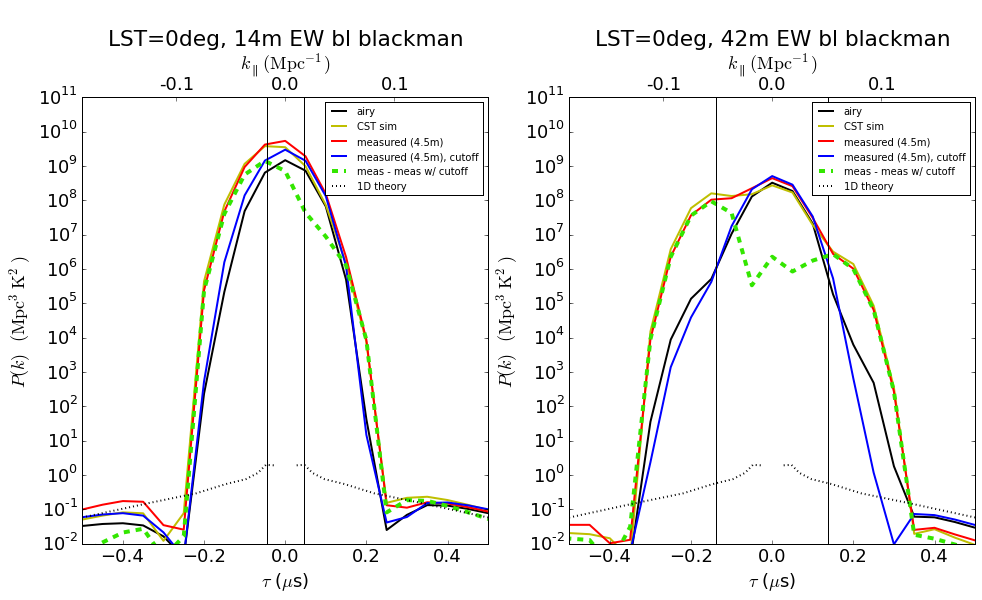
\includegraphics[width=6.7in]{LST0deg_14m_42m_EWbaselines_dish1_blackman.png}
%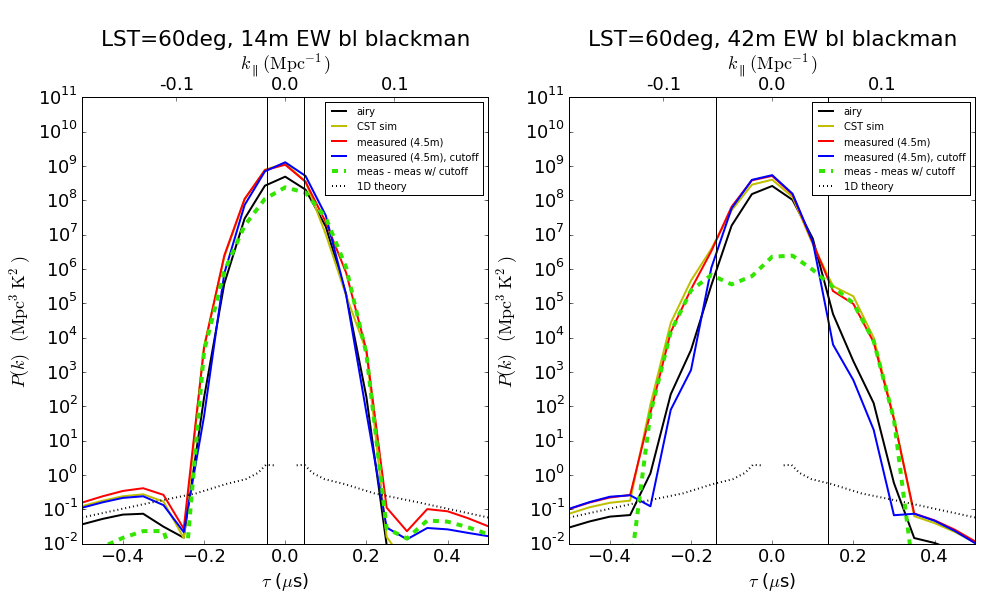
\includegraphics[width=6.7in]{LST60deg_14m_42m_EWbaselines_dish1_blackman.png}
%\caption{Simulated delay spectra for the GSM and point sources at $0^\circ$ (top pair) and $60^\circ$ (bottom pair) LST for EW baselines of length 14\,m (left pair) and 42\,m (right pair). The beams are are assumed constant over frequency.}
%\label{fig:delayspec}
%\end{figure*}

%\begin{figure*}[h]
%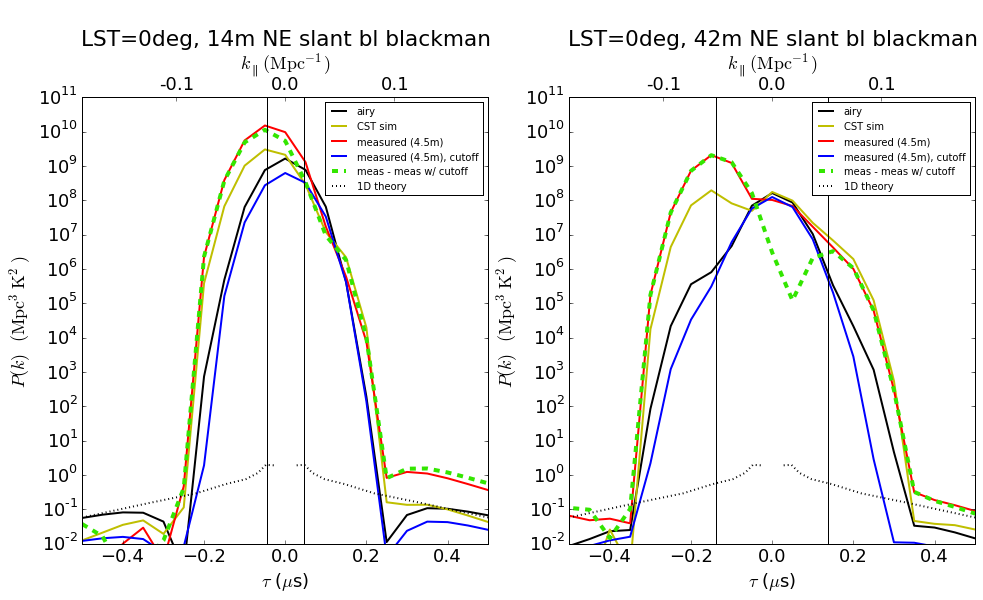
\includegraphics[width=6.7in]{LST0deg_14m_42m_NEslantbaselines_dish1_blackman.png}
%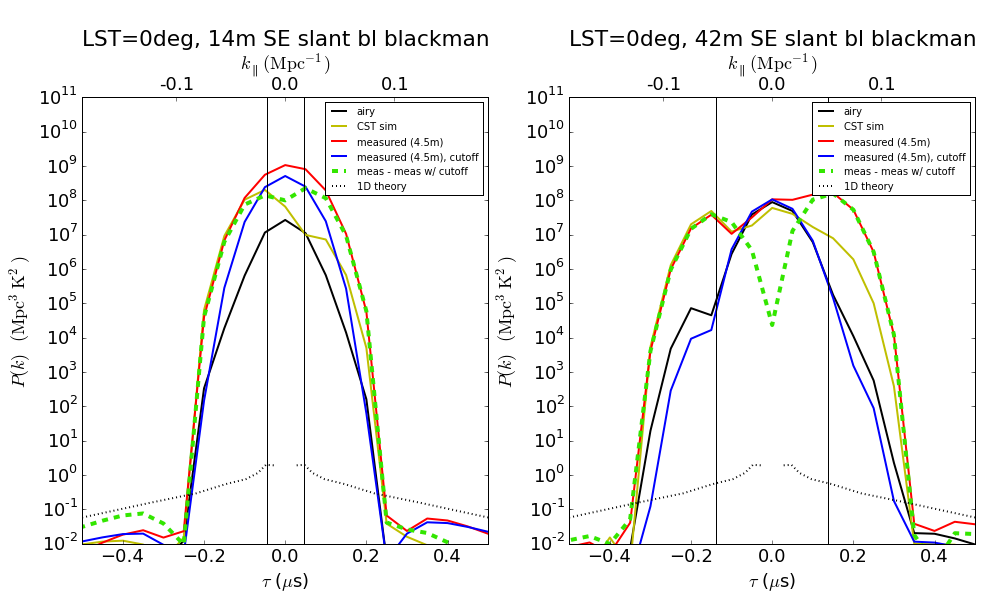
\includegraphics[width=6.7in]{LST0deg_14m_42m_SEslantbaselines_dish1_blackman.png}
%\caption{Simulated delay spectra for the GSM and point sources at $0^\circ$ LST for NE (top pair) and SE (bottom pair) baselines of length 14\,m (left pair) and 42\,m (right pair). The beams are are assumed constant over frequency.}
%\label{fig:delayspec2}
%\end{figure*}





\section{Discussion}

add stuff here







%% The reference list follows the main body and any appendices.
%% Use LaTeX's thebibliography environment to mark up your reference list.
%% Note \begin{thebibliography} is followed by an empty set of
%% curly braces.  If you forget this, LaTeX will generate the error
%% "Perhaps a missing \item?".
%%
%% thebibliography produces citations in the text using \bibitem-\cite
%% cross-referencing. Each reference is preceded by a
%% \bibitem command that defines in curly braces the KEY that corresponds
%% to the KEY in the \cite commands (see the first section above).
%% Make sure that you provide a unique KEY for every \bibitem or else the
%% paper will not LaTeX. The square brackets should contain
%% the citation text that LaTeX will insert in
%% place of the \cite commands.

%% We have used macros to produce journal name abbreviations.
%% AASTeX provides a number of these for the more frequently-cited journals.
%% See the Author Guide for a list of them.

%% Note that the style of the \bibitem labels (in []) is slightly
%% different from previous examples.  The natbib system solves a host
%% of citation expression problems, but it is necessary to clearly
%% delimit the year from the author name used in the citation.
%% See the natbib documentation for more details and options.

\bibliography{DishBeamMeasurements}


\end{document}
